\clearpage
\section{Results\label{sec:results}}

The likelihood described in Sec.~\ref{sec:likelihood} is used to
relate yields, uncertainties. It is constructed using Roofit
~\cite{roofit} and maximized using MINUIT~\cite{James:1975dr}, as
implemented in the package ra1stats~\cite{ra1stats}.

\subsection{Standard Model: background-only\label{sec:smInterp}}

To test the compatibility of the data with the Standard Model only hypothesis,
the signal term is removed from the likelihood model. The parameter values 
maximizing the likelihood function are listed in 
Tables~\ref{tab:mlParameterValues0b_le3j}--\ref{tab:mlParameterValues2b_ge4j}
found in Appendix~\ref{app:ml-params}. The resulting SM yields
along with the observed data yields are summarized in Tables~\ref{tab:ensemble-summary-posteriori}.
The uncertainty on the yields is obtained by constructing a probability density
function (p.d.f) from the maximized likelihood, then generating an
ensemble of pseudo-experiments from this p.d.f. and maximizing the same 
likelihood form for each pseudo-experiment, resulting in an ensemble of yields.
The $68\%$ quantile of each ensemble defines the quoted uncertainty on the 
corresponding yield.

\begin{center}
\begin{table}[h!]
  \caption{Summary of hadronic yields from fit.}
  \label{tab:ensemble-summary-posteriori}
  \centering
  \scriptsize
\begin{tabular}{ lllllllll }

\hline
& 375--475                       & 475--575                       & 575--675                       & 675--775                       & 775--875                       & 875--975                       & 975--1075                      & 1075--$\infty$                 \\ [1.000000ex]
\hline
0b, \njetlow, SM \T   & $2744^{+48}_{-43}$             & $771^{+21}_{-23}$              & $254^{+13}_{-13}$              & $76.5^{+6.1}_{-4.8}$           & $33.7^{+3.7}_{-3.8}$           & $11.8^{+1.9}_{-2.1}$           & $6.3^{+1.4}_{-1.3}$            & $3.2^{+1.0}_{-0.9}$            \\ 
0b, \njetlow, Data \T & $2728$                         & $766$                          & $257$                          & $77$                           & $32$                           & $9$                            & $9$                            & $4$                            \\ 
\hline
1b, \njetlow, SM \T   & $426^{+15}_{-17}$              & $114^{+6}_{-6}$                & $35.5^{+3.3}_{-2.8}$           & $10.1^{+1.4}_{-1.5}$           & $3.7^{+0.9}_{-0.8}$            & $1.6^{+0.7}_{-0.6}$            & $0.5^{+0.3}_{-0.4}$            & $0.1^{+0.1}_{-0.0}$            \\ 
1b, \njetlow, Data \T & $444$                          & $118$                          & $36$                           & $15$                           & $3$                            & $2$                            & $1$                            & $0$                            \\ 
\hline
2b, \njetlow, SM \T   & $65.0^{+4.3}_{-4.3}$           & $18.4^{+1.7}_{-1.6}$           & $4.2^{+0.6}_{-0.5}$            & $1.1^{+0.3}_{-0.2}$            & $0.2^{+0.1}_{-0.1}$            & $0.0^{+0.0}_{-0.0}$            & $0.0^{+0.0}_{-0.0}$            & $0.0^{+0.0}_{-0.0}$            \\ 
2b, \njetlow, Data \T & $78$                           & $18$                           & $8$                            & $3$                            & $0$                            & $0$                            & $0$                            & $0$                            \\ 
\hline
0b, \njethigh, SM \T   & $456^{+15}_{-14}$              & $291^{+12}_{-12}$              & $148^{+8}_{-7}$                & $66.0^{+5.6}_{-5.2}$           & $27.1^{+2.9}_{-3.4}$           & $14.0^{+1.9}_{-2.1}$           & $6.5^{+1.5}_{-1.2}$            & $3.2^{+1.0}_{-0.9}$            \\ 
0b, \njethigh, Data \T & $480$                          & $299$                          & $158$                          & $66$                           & $28$                           & $15$                           & $6$                            & $2$                            \\ 
\hline
1b, \njethigh, SM \T   & $190^{+10}_{-8}$               & $120^{+6}_{-5}$                & $45.6^{+3.1}_{-3.8}$           & $17.1^{+2.6}_{-1.9}$           & $6.8^{+1.5}_{-1.3}$            & $5.4^{+1.3}_{-1.6}$            & $2.4^{+0.9}_{-0.9}$            & $1.2^{+0.7}_{-0.8}$            \\ 
1b, \njethigh, Data \T & $206$                          & $135$                          & $45$                           & $14$                           & $8$                            & $6$                            & $2$                            & $0$                            \\ 
\hline
2b, \njethigh, SM \T   & $73.6^{+4.2}_{-4.2}$           & $45.7^{+2.8}_{-2.9}$           & $20.4^{+1.8}_{-1.8}$           & $7.7^{+1.2}_{-1.0}$            & $1.9^{+0.3}_{-0.3}$            & $0.9^{+0.2}_{-0.2}$            & $0.4^{+0.1}_{-0.1}$            & $0.4^{+0.1}_{-0.2}$            \\ 
2b, \njethigh, Data \T & $79$                           & $52$                           & $31$                           & $12$                           & $1$                            & $2$                            & $0$                            & $1$                            \\ 
\hline
  \end{tabular}
\end{table}
\end{center}

Figures~\ref{fig:best-fit-le3j0b}--\ref{fig:best-fit-ge4j2b} show
the \scalht-binned observed data yields (black filled circles) and the
SM expectations and uncertainties (dark blue solid line with light
blue bands) as determined by the fit for the hadronic signal region
and the \mj or both (\mj,\gj) control samples, depending on the event
category. The uncertainties in the SM expectations obtained from the 
ensemble of pseudo-experiments (shown in shaded bands) reflect the statistical uncertainties in
the considered data samples and the systematic uncertainties
in the transfer factors as discussed in Section~\ref{sec:bkgd-syst}.
Figures~\ref{fig:best-fit-le3j0b}--\ref{fig:best-fit-ge4j2b} are summarized
in tabular format in Tables~\ref{tab:ensemble-0b le3j}--\ref{tab:ensemble-2b ge4j} 
in Appendix~\ref{app:ml-yields} along with observed data yields and the fit 
result for all event categories and both signal region and control sample bins.

For each \nb, \njet category, the goodness-of-fit of the SM-only hypothesis 
is determined by considering simultaneously all \scalht bins entering
the likelihood. The goodness-of-fit described in Ref.~\cite{Cowan:358560} is obtained
by comparing the nominal maximized likelihood value \lk{data}{max} to 
the corresponding ensemble of values, \lk{}{max}. The quantile in which \lk{data}{max}
falls in the distributions is interpreted as a p-value.  A p-value derived from
a chi-square is also plotted for comparison. 

The p-values obtained, shown in Figure~\ref{fig:fluct} (a), are found 
to be uniformly distributed in the range 0.0--1.0, with the lowest p-value
determined to be 0.06.

The compatibility of the SM expectation and observed event count is
also evaluated for each of the 48 hadronic search bins. A profile
likelihood ratio is used to determine a p-value and the pull per
signal region bin. Figure~\ref{fig:sigVsCat} shows the pull as a function
of the signal region bin (Right). In general the SM-only hypotheses
agrees well with data, though there are mild excesses (i.e. $> 1.5\sigma$)
in the $\nb = 1$ and $\nb = 2$ bins where the most pronounced excess is in
the $\njethigh, \nb = 2, 575 < \scalht < 675~\GeV$ bin, with 2.4$\sigma$. This
bin as been carefully studied to try to determine the source of the excess
in the data.  There is no obvious discrepancy in any specific kinematic region
(jet $\pt$, $\scalht$, $\met$, ... ), or from one source of background in particular.
In summary, an excess greater that 2$\sigma$ in one of 48 search bins is consistent with 
an, albeit rare, statistical fluctuation.

\begin{figure}[h!]
  \begin{center}
    \subfigure[p-values per event category.]{
      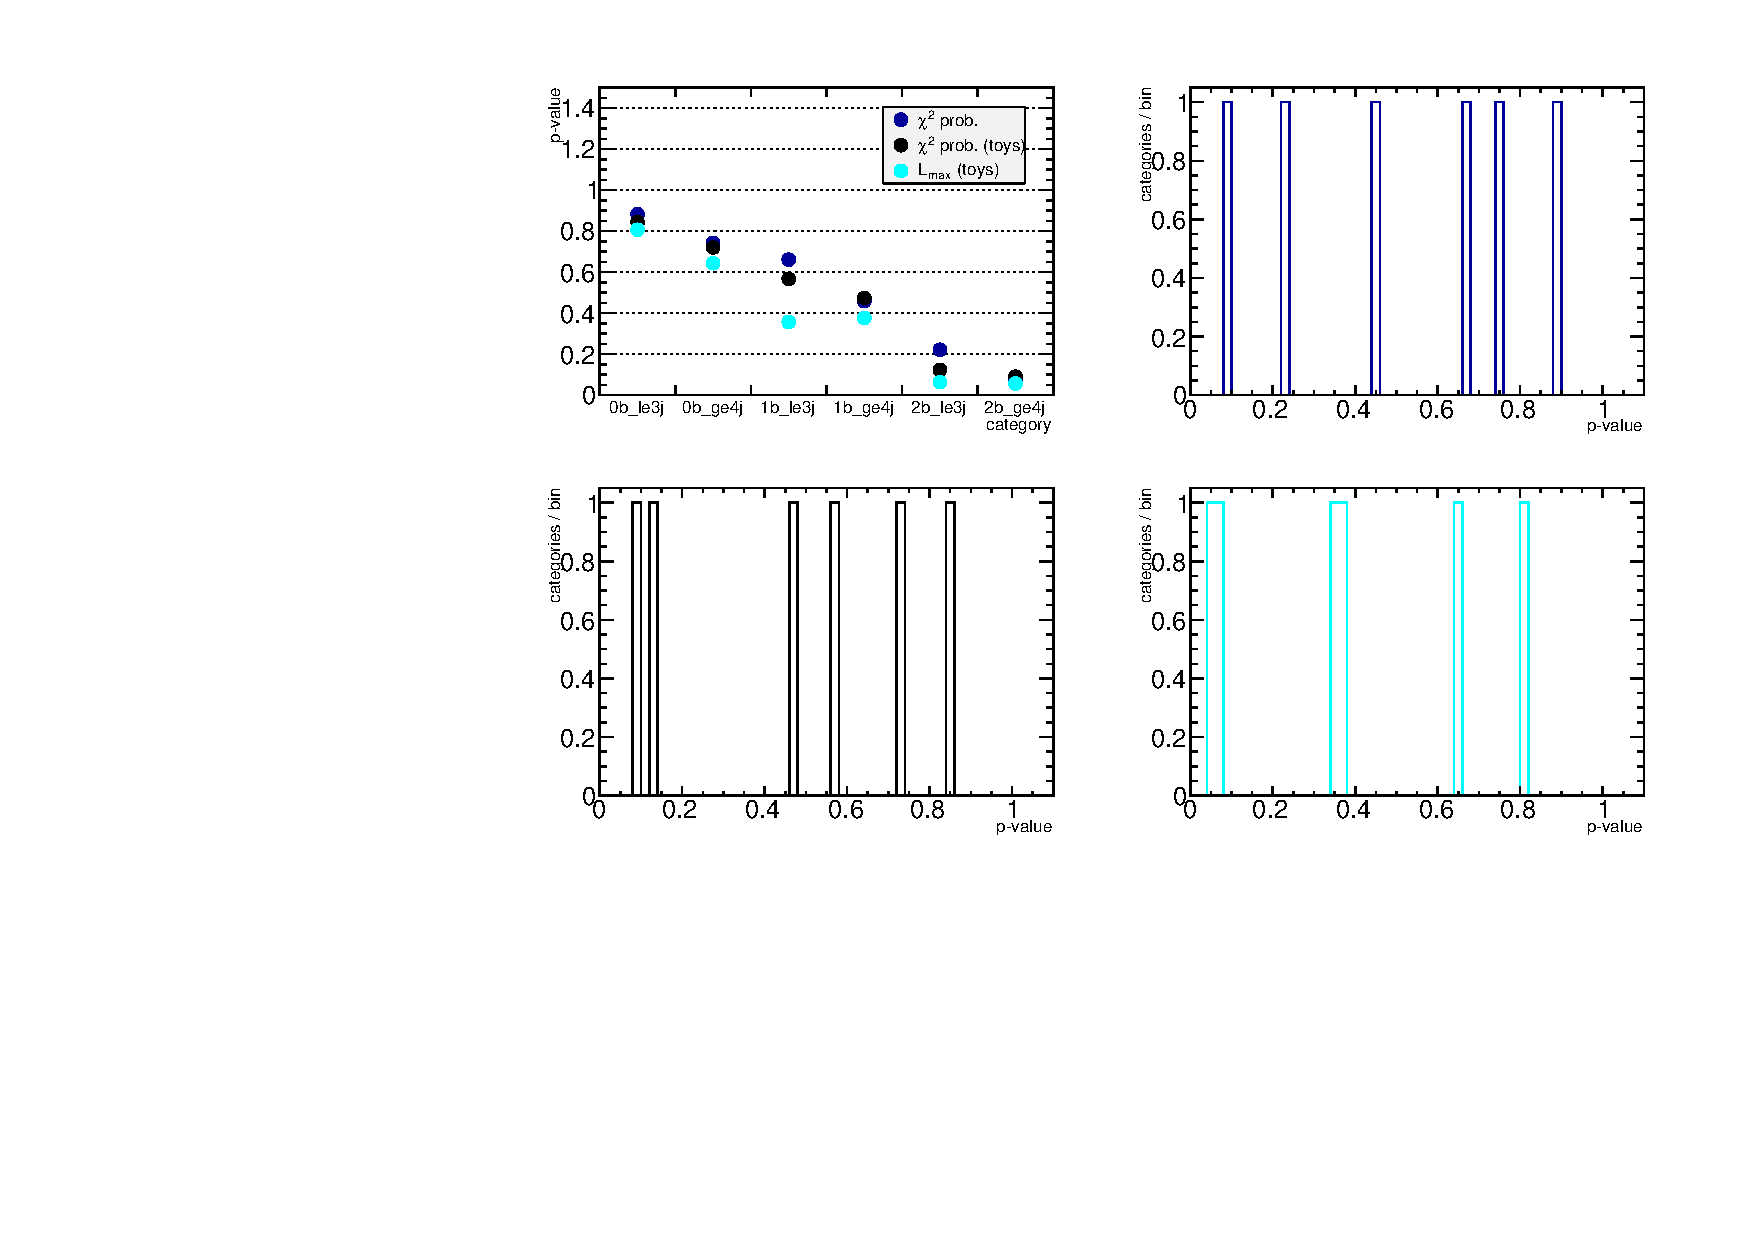
\includegraphics[width=0.75\textwidth, trim=0 190 290 20, clip=true]{figures/fit/v22/pValues} % lbrt
    } \\
    \subfigure[Pull versus signal region bin.\label{fig:sigVsCat}]{
      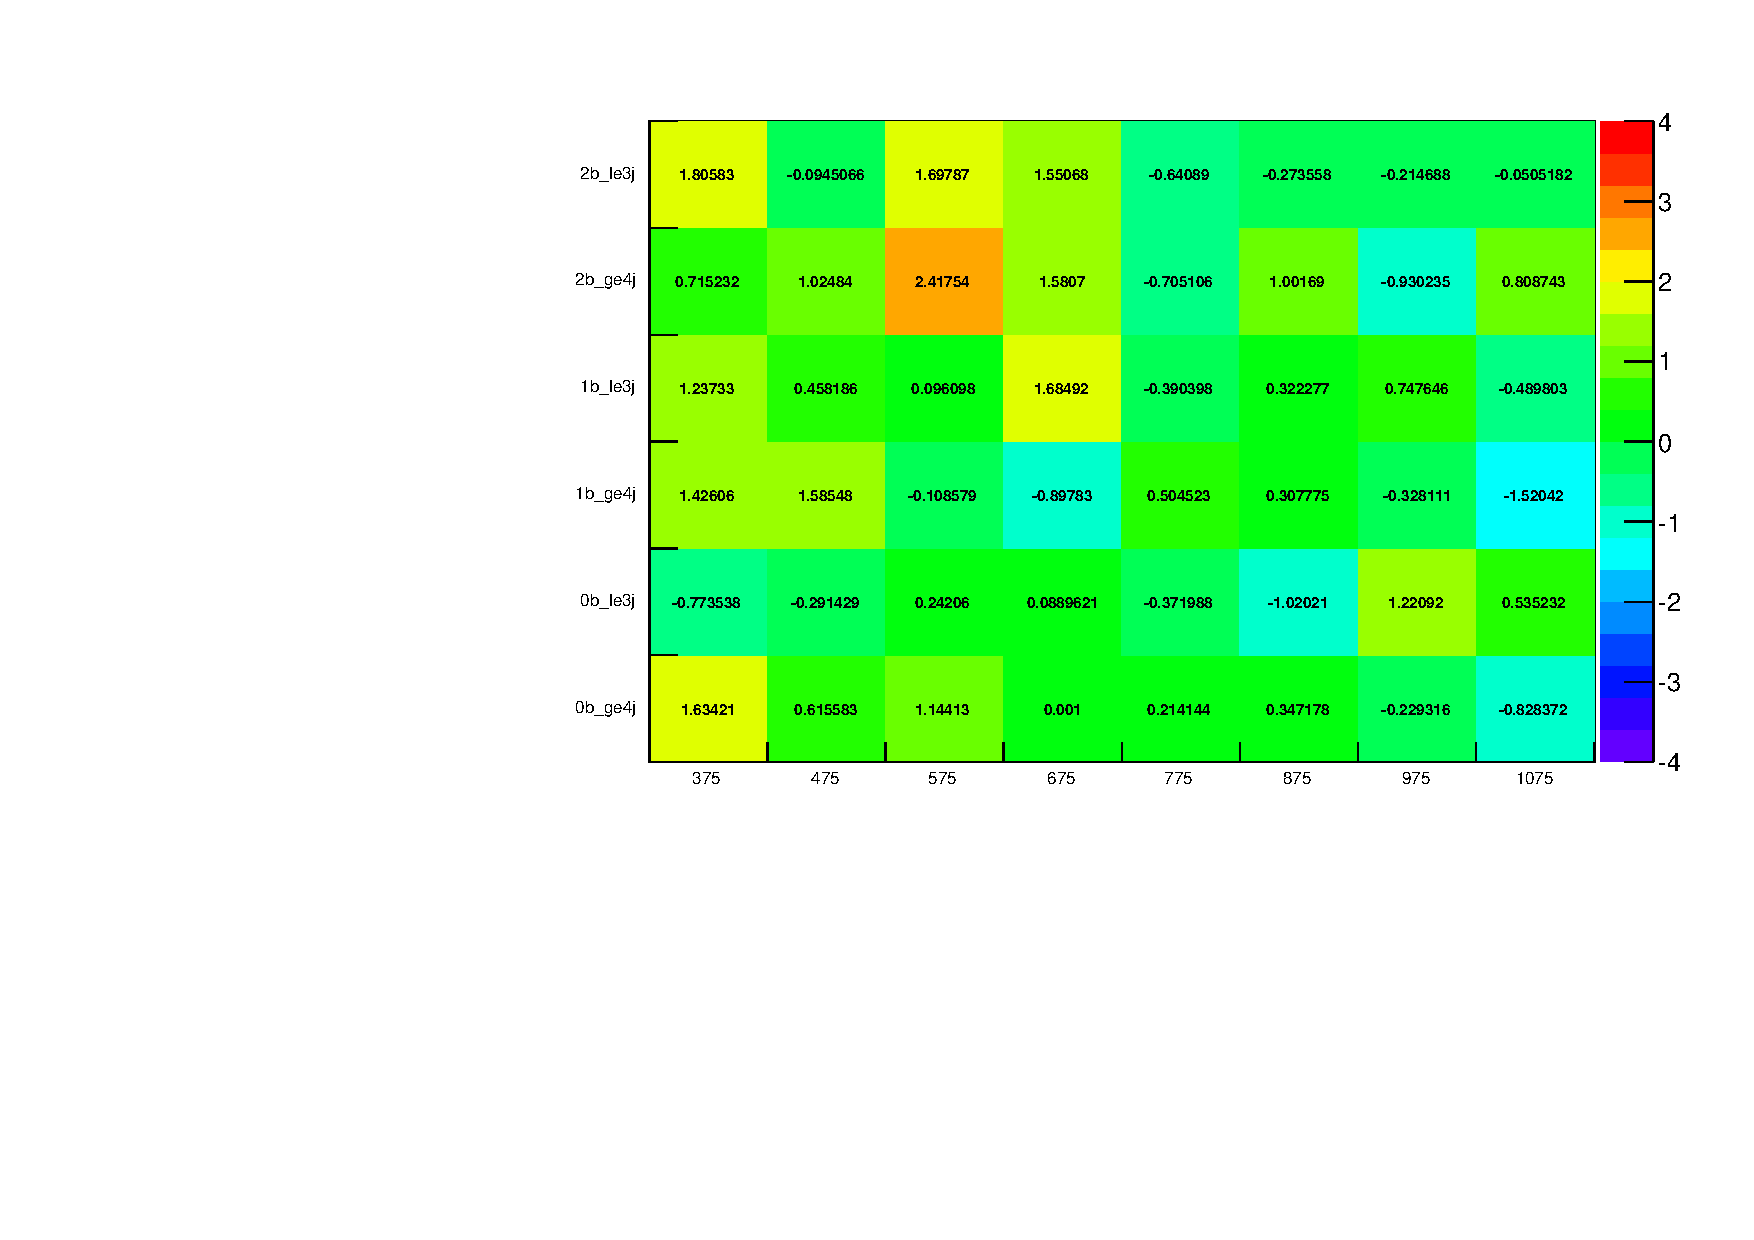
\includegraphics[width=0.75\textwidth, trim=0 0 0 30, clip=true]{figures/fit/v22/significances_catVsHt}
    } \\
%    \subfigure[Pull per signal region bin.]{
%      \includegraphics[width=0.45\textwidth, trim=0 0 0 0, clip=true]{figures/fit/v1/pull_per_bin_gaus}
%    } 
%    \subfigure[p-value per signal region bin.]{
%      \includegraphics[width=0.45\textwidth, trim=0 0 0 0, clip=true]{figures/fit/v1/pvalue_per_bin}
%    } \\
    \caption{Pulls and p-values. See text for details}
    \label{fig:fluct}
  \end{center}
\end{figure}

%Figures~\ref{fig:best-fit-control-only-le3j0b}--\ref{fig:best-fit-control-only-ge4jge4b}
%show the observed data yields (black filled circles) and SM
%expectations and associated uncertainties (dark green solid line with
%light green bands). In this case, the hadronic signal region yields
%are not considered and the SM predictions are determined solely from
%the \mj or all three data control samples (depending on the event
%category). Figures~\ref{fig:best-fit-control-only-le3j0b}--\ref{fig:best-fit-control-only-ge4jge4b}
%and Figures~\ref{fig:best-fit-le3j0b}--\ref{fig:best-fit-ge4jge4b}
%correspond to ``a priori'' and ``a posteriori'' fits, respectively.
%In addition, Table~\ref{tab:ensemble-summary-priori} summarises the
%observed data yields and the fit result for all event categories and
%all signal region bins for the ``a priori'' fit.  The uncertainties in
%the SM expectations are smaller for the ``a posteriori'' fit due to
%the additional information from hadronic signal region counts.
%

%\begin{landscape}
%\begin{center}
%\begin{table}[h!]
%  \caption{Summary of the ``a priori'' fit.}
%  \label{tab:ensemble-summary-priori}
%  \centering
%  \scriptsize
%  \begin{tabular}{ llllllllllllll }
%    \hline
%    \hline
%    \multicolumn{2}{c}{} & \multicolumn{11}{c}{\scalht (GeV)}                                                                                                                                                                                                                                              \\ 
%    \njet                & \nb      &        & 200--275              & 275--325             & 325--375              & 375--475             & 475--575              & 575--675             & 675--775             & 775--875             & 875--975             & 975--1075           & 1075--$\infty$      \\ 
%    \hline
%    2--3                 & $0$      & SM\T   & $12391^{+368}_{-325}$ & $5566^{+325}_{-188}$ & $3424^{+205}_{-149}$  & $2473^{+131}_{-96}$  & $684^{+38}_{-34}$     & $231^{+18}_{-19}$    & $69.8^{+6.1}_{-6.6}$ & $27.9^{+3.9}_{-3.2}$ & $11.0^{+2.1}_{-1.8}$ & $5.4^{+0.8}_{-1.0}$ & $3.7^{+0.9}_{-0.8}$ \\ 
%    2--3                 & $0$      & Data\T & $13310$               & $5404$               & $3580$                & $2475$               & $698$                 & $224$                & $81$                 & $28$                 & $12$                 & $9$                 & $3$                 \\ 
%    2--3                 & $1$      & SM\T   & $1626^{+60}_{-47}$    & $862^{+48}_{-41}$    & $548^{+29}_{-35}$     & $413^{+28}_{-23}$    & $103^{+8}_{-7}$       & $26.6^{+3.1}_{-3.2}$ & $9.5^{+1.2}_{-1.6}$  & $3.1^{+0.9}_{-0.8}$  & $2.6^{+0.9}_{-0.8}$  & $0.4^{+0.2}_{-0.2}$ & $0.2^{+0.1}_{-0.1}$ \\ 
%    2--3                 & $1$      & Data\T & $1802$                & $835$                & $597$                 & $416$                & $97$                  & $29$                 & $7$                  & $4$                  & $1$                  & $0$                 & $0$                 \\ 
%    2--3                 & $2$      & SM\T   & $177^{+9}_{-7}$       & $113^{+7}_{-7}$      & $97.3^{+6.3}_{-6.6}$  & $66.0^{+6.3}_{-5.8}$ & $14.6^{+1.7}_{-1.4}$  & $2.9^{+0.5}_{-0.5}$  & $1.1^{+0.2}_{-0.3}$  & $0.2^{+0.1}_{-0.1}$  & $0.1^{+0.1}_{-0.0}$  & \multicolumn{2}{c}{}                      \\ 
%    2--3                 & $2$      & Data\T & $174$                 & $119$                & $117$                 & $70$                 & $18$                  & $7$                  & $1$                  & $0$                  & $0$                  & \multicolumn{2}{c}{}                      \\ 
%    $\geq 4$             & $0$      & SM\T   & $106^{+10}_{-10}$     & $520^{+32}_{-34}$    & $448^{+39}_{-54}$     & $369^{+31}_{-25}$    & $224^{+17}_{-15}$     & $109^{+14}_{-13}$    & $46.8^{+5.8}_{-6.1}$ & $19.2^{+2.8}_{-2.7}$ & $9.2^{+1.7}_{-1.7}$  & $3.7^{+1.1}_{-0.9}$ & $3.2^{+0.7}_{-0.7}$ \\ 
%    $\geq 4$             & $0$      & Data\T & $103$                 & $590$                & $455$                 & $391$                & $274$                 & $149$                & $56$                 & $18$                 & $12$                 & $7$                 & $8$                 \\ 
%    $\geq 4$             & $1$      & SM\T   & $39.8^{+3.2}_{-3.5}$  & $223^{+14}_{-12}$    & $211^{+25}_{-23}$     & $171^{+18}_{-15}$    & $98.7^{+10.1}_{-9.1}$ & $35.5^{+6.0}_{-5.1}$ & $14.8^{+2.2}_{-2.2}$ & $6.8^{+1.5}_{-1.2}$  & $3.2^{+0.9}_{-0.9}$  & $1.1^{+0.5}_{-0.4}$ & $1.2^{+0.4}_{-0.4}$ \\ 
%    $\geq 4$             & $1$      & Data\T & $38$                  & $207$                & $250$                 & $181$                & $108$                 & $41$                 & $10$                 & $14$                 & $6$                  & $1$                 & $1$                 \\ 
%    $\geq 4$             & $2$      & SM\T   & $13.0^{+1.0}_{-0.9}$  & $75.5^{+4.8}_{-4.8}$ & $96.1^{+11.4}_{-9.4}$ & $69.5^{+7.2}_{-8.3}$ & $43.9^{+4.8}_{-5.7}$  & $16.1^{+3.7}_{-2.7}$ & $5.2^{+1.2}_{-0.9}$  & $1.7^{+0.3}_{-0.4}$  & $1.9^{+0.5}_{-0.4}$  & \multicolumn{2}{c}{}                      \\ 
%    $\geq 4$             & $2$      & Data\T & $17$                  & $82$                 & $95$                  & $86$                 & $48$                  & $19$                 & $10$                 & $2$                  & $1$                  & \multicolumn{2}{c}{}                      \\ 
%    $\geq 4$             & $3$      & SM\T   & $1.0^{+0.2}_{-0.2}$   & $8.1^{+0.8}_{-0.8}$  & $11.7^{+1.9}_{-1.6}$  & $8.0^{+1.4}_{-1.2}$  & $5.3^{+1.2}_{-0.8}$   & $2.3^{+0.6}_{-0.5}$  & $0.8^{+0.2}_{-0.2}$  & $0.2^{+0.1}_{-0.1}$  & $0.2^{+0.1}_{-0.1}$  & \multicolumn{2}{c}{}                      \\ 
%    $\geq 4$             & $3$      & Data\T & $0$                   & $9$                  & $8$                   & $8$                  & $9$                   & $1$                  & $3$                  & $0$                  & $0$                  & \multicolumn{2}{c}{}                      \\ 
%    $\geq 4$             & $\geq 4$ & SM\T   & $0.0^{+0.0}_{-0.0}$  & $0.1^{+0.1}_{-0.1}$  & $0.6^{+0.3}_{-0.3}$   & $0.7^{+0.3}_{-0.3}$  & \multicolumn{7}{l}{}                                                                                                                                          \\ 
%    $\geq 4$             & $\geq 4$ & Data\T & $0$                   & $0$                  & $0$                   & $3$                  & \multicolumn{7}{l}{}                                                                                                                                          \\ 
%    \hline
%    \hline
%  \end{tabular}
%\end{table}
%\end{center}
%\end{landscape}
%
\clearpage
\begin{figure}[t!]
  \begin{center}
    \subfigure[Hadronic sample (linear scale)]{
      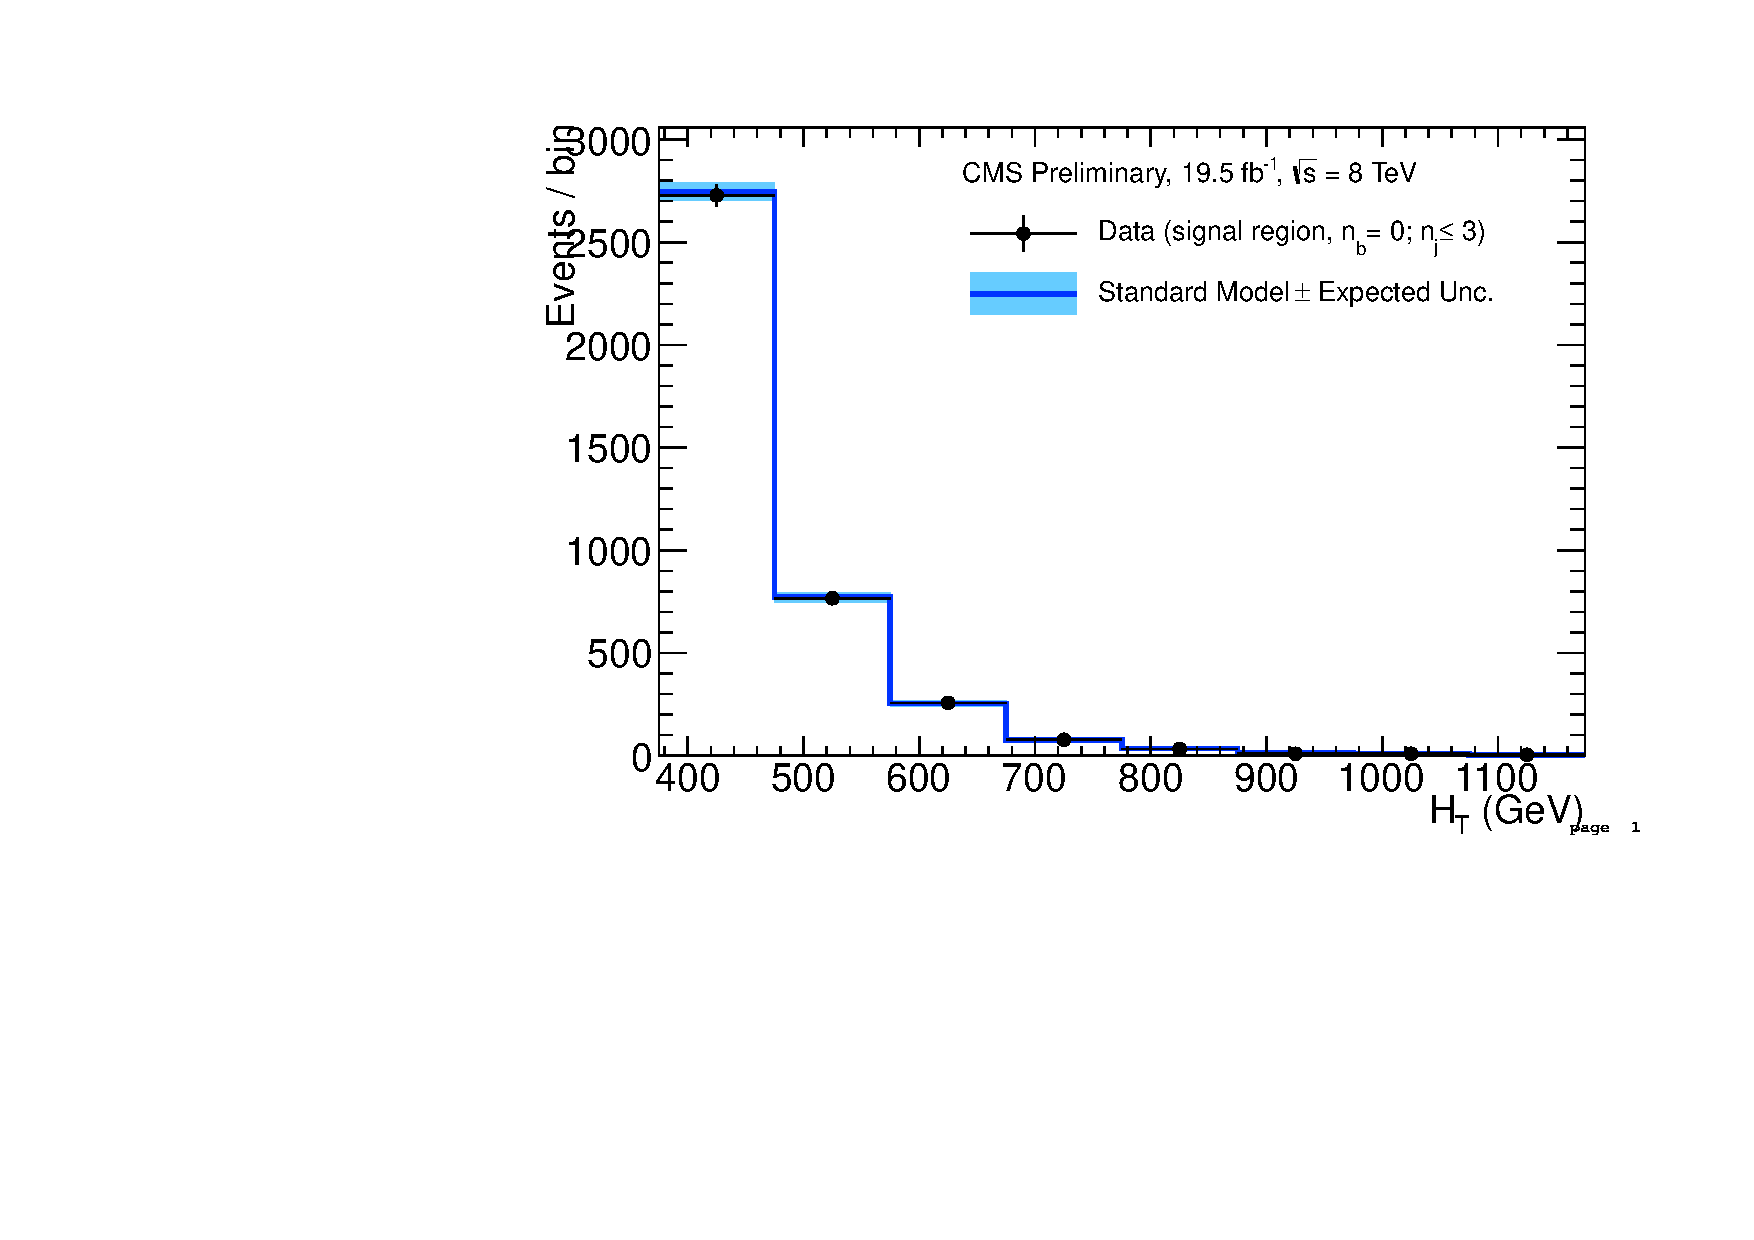
\includegraphics[width=0.45\textwidth,page=1]{figures/fit/v22/bestFit_2012pf_RQcdZero_fZinvAll_0b_le3j-1hp_smOnly}
    } 
    \subfigure[Hadronic sample (logarithmic scale)]{
      \includegraphics[width=0.45\textwidth,page=2]{figures/fit/v22/bestFit_2012pf_RQcdZero_fZinvAll_0b_le3j-1hp_smOnly}
    } \\
    \subfigure[$\mu$ + jets sample]{
      \includegraphics[width=0.45\textwidth,page=4]{figures/fit/v22/bestFit_2012pf_RQcdZero_fZinvAll_0b_le3j-1hp_smOnly}
    } 
    \subfigure[$\gamma$ + jets sample]{
      \includegraphics[width=0.45\textwidth,page=6]{figures/fit/v22/bestFit_2012pf_RQcdZero_fZinvAll_0b_le3j-1hp_smOnly}
    } 
    \caption{\label{fig:best-fit-le3j0b} Comparison of the
      \scalht-binned observed data yields and SM expectations when
      requiring \njetlow and $\nb = 0$ for the (a-b) hadronic, (c)
      \mj, (d) \mmj and (e) \gj samples, as determined by a
      simultaneous fit to all data samples under the SM-only
      hypothesis. The observed event yields in data (black dots) and
      the expectations and their uncertainties (dark blue solid line
      with light blue bands), as determined by the simultaneous fit,
      are shown. %For illustrative purposes only, the signal
      %expectations (pink dashed line) for the model \texttt{T2cc} with
      %$m_{\sq} = 250\GeV$ and $m_{\text{LSP}} = 240\GeV$ are stacked
      %on top of the SM expectations.
      }
  \end{center}
\end{figure}

\clearpage
\begin{figure}[t!]
  \begin{center}
    \subfigure[Hadronic sample (linear scale)]{
      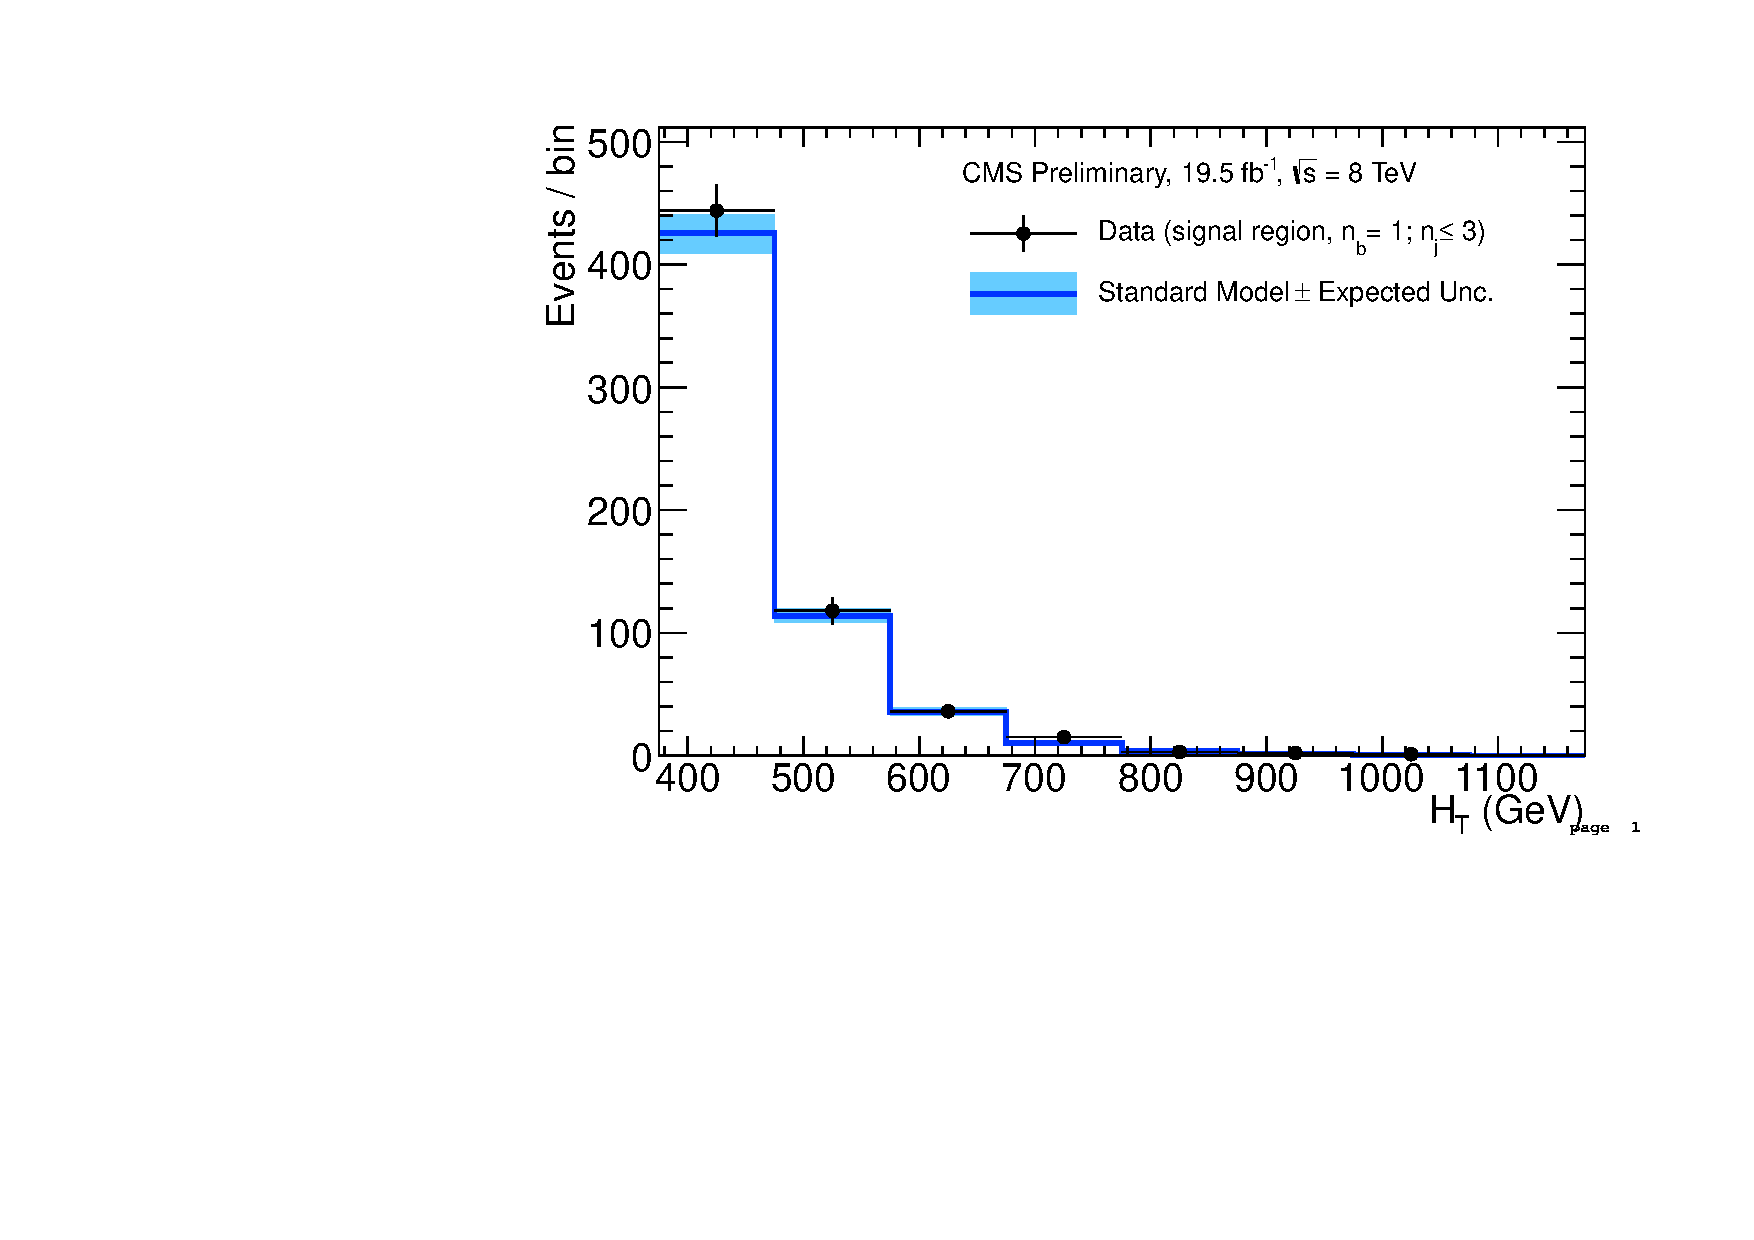
\includegraphics[width=0.45\textwidth,page=1]{figures/fit/v22/bestFit_2012pf_RQcdZero_fZinvAll_1b_le3j-1hp_smOnly}
    } 
    \subfigure[Hadronic sample (logarithmic scale)]{
      \includegraphics[width=0.45\textwidth,page=2]{figures/fit/v22/bestFit_2012pf_RQcdZero_fZinvAll_1b_le3j-1hp_smOnly}
    } \\
    \subfigure[$\mu$ + jets sample]{
      \includegraphics[width=0.45\textwidth,page=4]{figures/fit/v22/bestFit_2012pf_RQcdZero_fZinvAll_1b_le3j-1hp_smOnly}
    } 
    \subfigure[$\gamma$ + jets sample]{
      \includegraphics[width=0.45\textwidth,page=6]{figures/fit/v22/bestFit_2012pf_RQcdZero_fZinvAll_1b_le3j-1hp_smOnly}
    } 
    \caption{\label{fig:best-fit-le3j1b} Comparison of the
      \scalht-binned observed data yields and SM expectations when
      requiring \njetlow and $\nb = 1$ for the (a-b) hadronic, (c)
      \mj, (d) \mmj and (e) \gj samples, as determined by a
      simultaneous fit to all data samples under the SM-only
      hypothesis. The observed event yields in data (black dots) and
      the expectations and their uncertainties (dark blue solid line
      with light blue bands), as determined by the simultaneous fit,
      are shown. %For illustrative purposes only, the signal
      %expectations (pink dashed line) for the model \texttt{T2cc} with
      %$m_{\sq} = 250\GeV$ and $m_{\text{LSP}} = 170\GeV$ are stacked
      %on top of the SM expectations.
      }
  \end{center}
\end{figure}

\clearpage
\begin{figure}[t!]
  \begin{center}
    \subfigure[Hadronic sample (linear scale)]{
      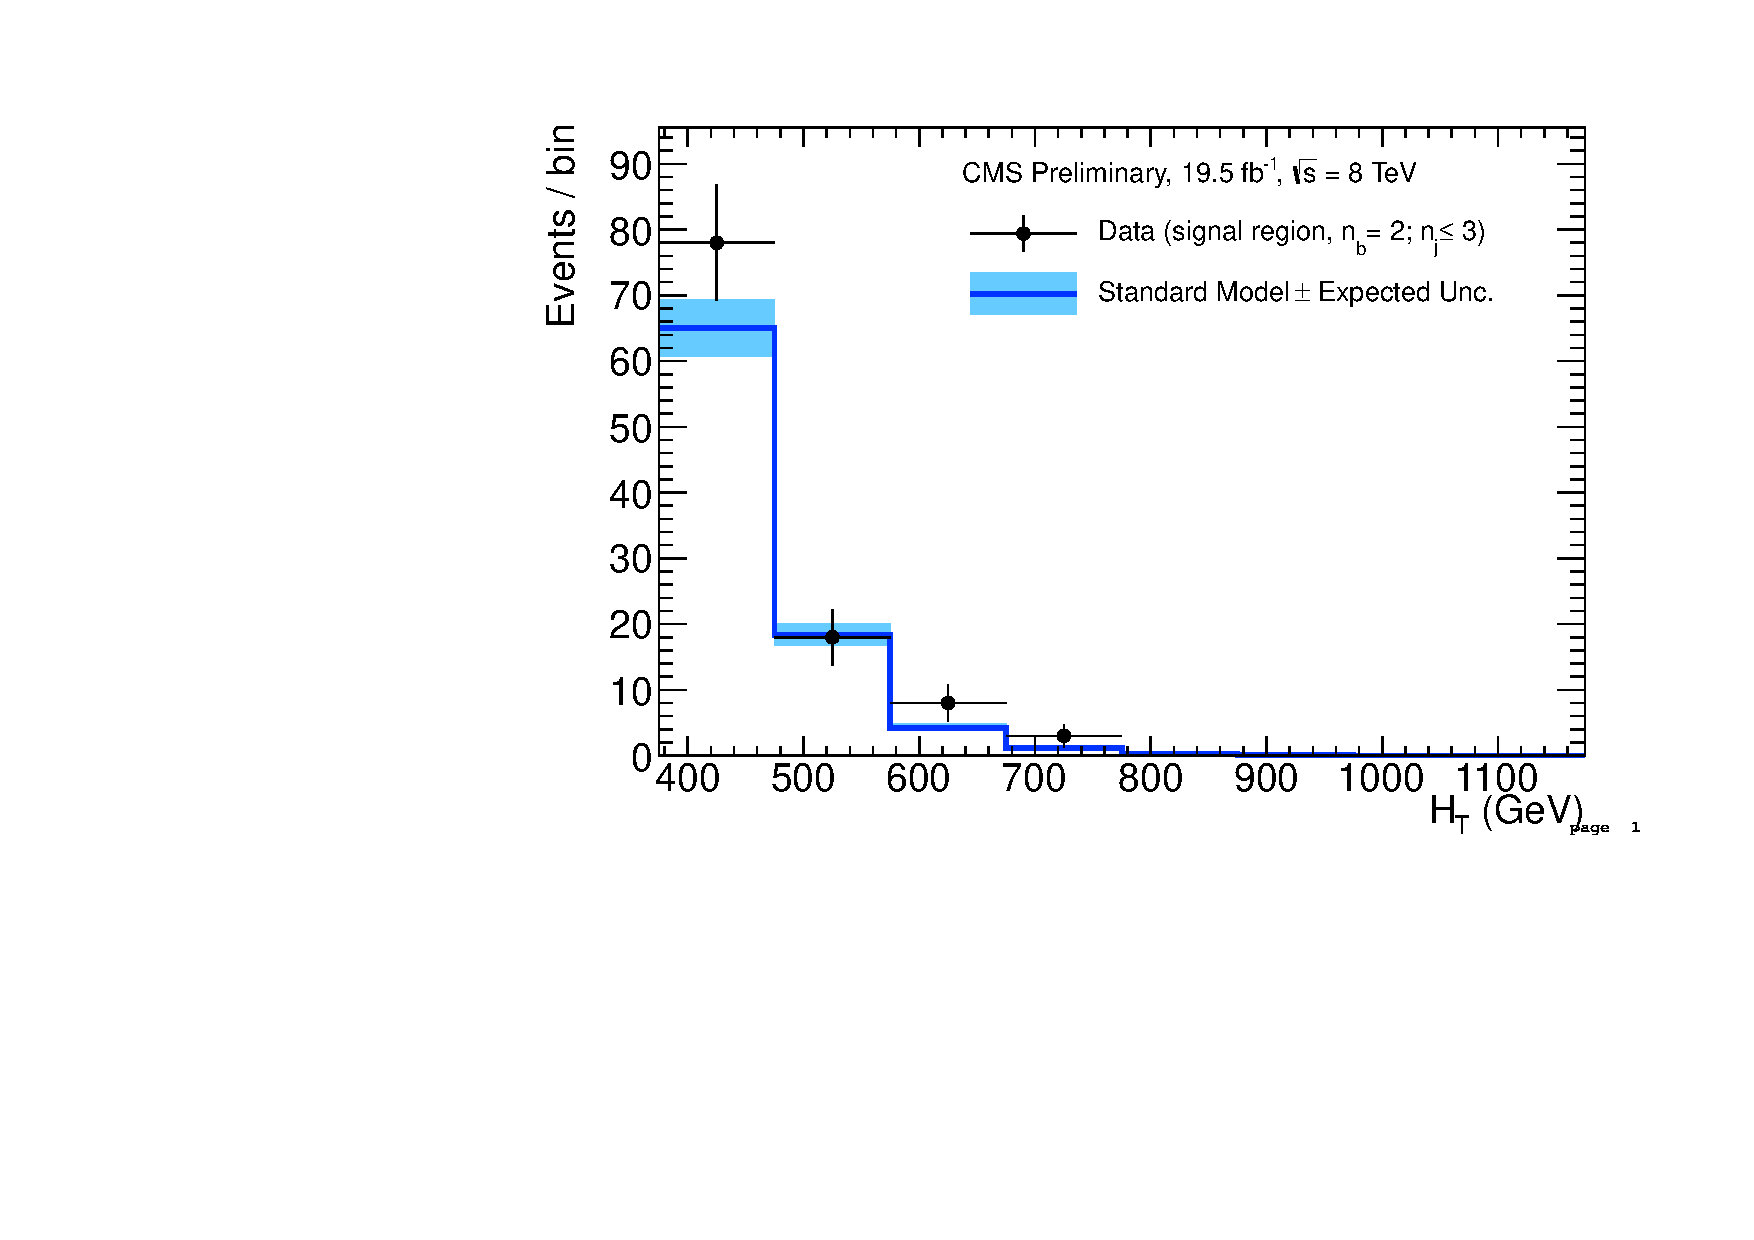
\includegraphics[width=0.45\textwidth,page=1]{figures/fit/v22/bestFit_2012pf_RQcdZero_fZinvAll_2b_le3j-1h_smOnly}
    } 
    \subfigure[Hadronic sample (logarithmic scale)]{
      \includegraphics[width=0.45\textwidth,page=2]{figures/fit/v22/bestFit_2012pf_RQcdZero_fZinvAll_2b_le3j-1h_smOnly}
    } \\
    \subfigure[$\mu$ + jets sample]{
      \includegraphics[width=0.45\textwidth,page=4]{figures/fit/v22/bestFit_2012pf_RQcdZero_fZinvAll_2b_le3j-1h_smOnly}
    } 
    \caption{\label{fig:best-fit-le3j2b} Comparison of the
      \scalht-binned observed data yields and SM expectations when
      requiring \njetlow and $\nb = 2$ for the (a-b) hadronic and \mj
      samples, as determined by a simultaneous fit to both the
      hadronic and \mj data samples under the SM-only hypothesis. The
      observed event yields in data (black dots) and the expectations
      and their uncertainties (dark blue solid line with light blue
      bands), as determined by the simultaneous fit, are shown. }
%      For illustrative purposes only, the signal expectations (pink
%      dashed line) for the model \texttt{T2cc} with $m_{\sq} =
%      250\GeV$ and $m_{\text{LSP}} = 240\GeV$ are stacked on top of
%      the SM expectations.}
  \end{center}
\end{figure}

\clearpage
\begin{figure}[t!]
  \begin{center}
    \subfigure[Hadronic sample (linear scale)]{
      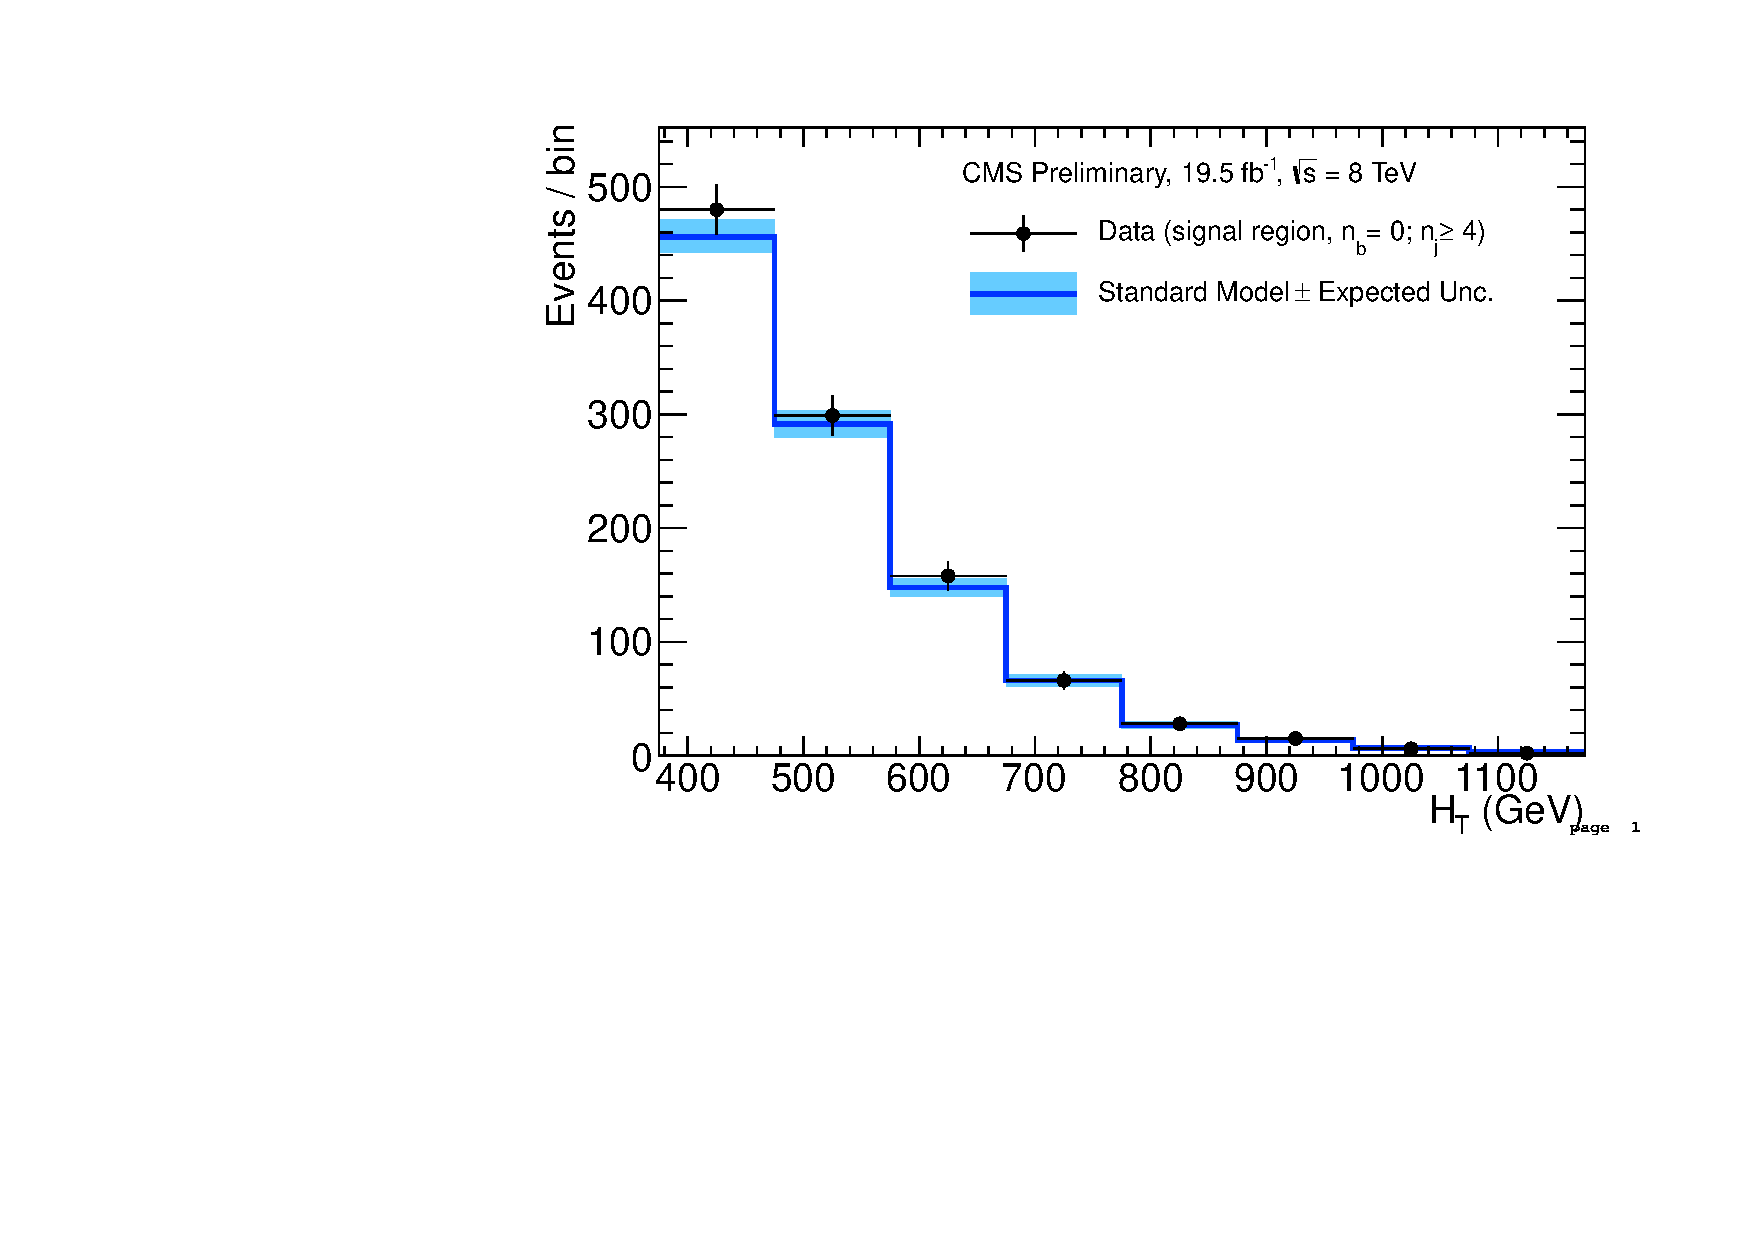
\includegraphics[width=0.45\textwidth,page=1]{figures/fit/v22/bestFit_2012pf_RQcdZero_fZinvAll_0b_ge4j-1hp_smOnly}
    } 
    \subfigure[Hadronic sample (logarithmic scale)]{
      \includegraphics[width=0.45\textwidth,page=2]{figures/fit/v22/bestFit_2012pf_RQcdZero_fZinvAll_0b_ge4j-1hp_smOnly}
    } \\
    \subfigure[$\mu$ + jets sample]{
      \includegraphics[width=0.45\textwidth,page=4]{figures/fit/v22/bestFit_2012pf_RQcdZero_fZinvAll_0b_ge4j-1hp_smOnly}
    } 
    \subfigure[$\gamma$ + jets sample]{
      \includegraphics[width=0.45\textwidth,page=6]{figures/fit/v22/bestFit_2012pf_RQcdZero_fZinvAll_0b_ge4j-1hp_smOnly}
    } 
    \caption{\label{fig:best-fit-ge4j0b} Comparison of the
      \scalht-binned observed data yields and SM expectations when
      requiring \njethigh and $\nb = 0$ for the (a-b) hadronic, (c)
      \mj, (d) \mmj and (e) \gj samples, as determined by a
      simultaneous fit to all data samples under the SM-only
      hypothesis. The observed event yields in data (black dots) and
      the expectations and their uncertainties (dark blue solid line
      with light blue bands), as determined by the simultaneous fit,
      are shown. 
      %For illustrative purposes only, the signal
      %expectations (pink dashed line) for the model \texttt{T2cc} with
      %$m_{\sq} = 250\GeV$ and $m_{\text{LSP}} = 170\GeV$ are stacked
      %on top of the SM expectations.
      }
  \end{center}
\end{figure}

\clearpage
\begin{figure}[t!]
  \begin{center}
    \subfigure[Hadronic sample (linear scale)]{
      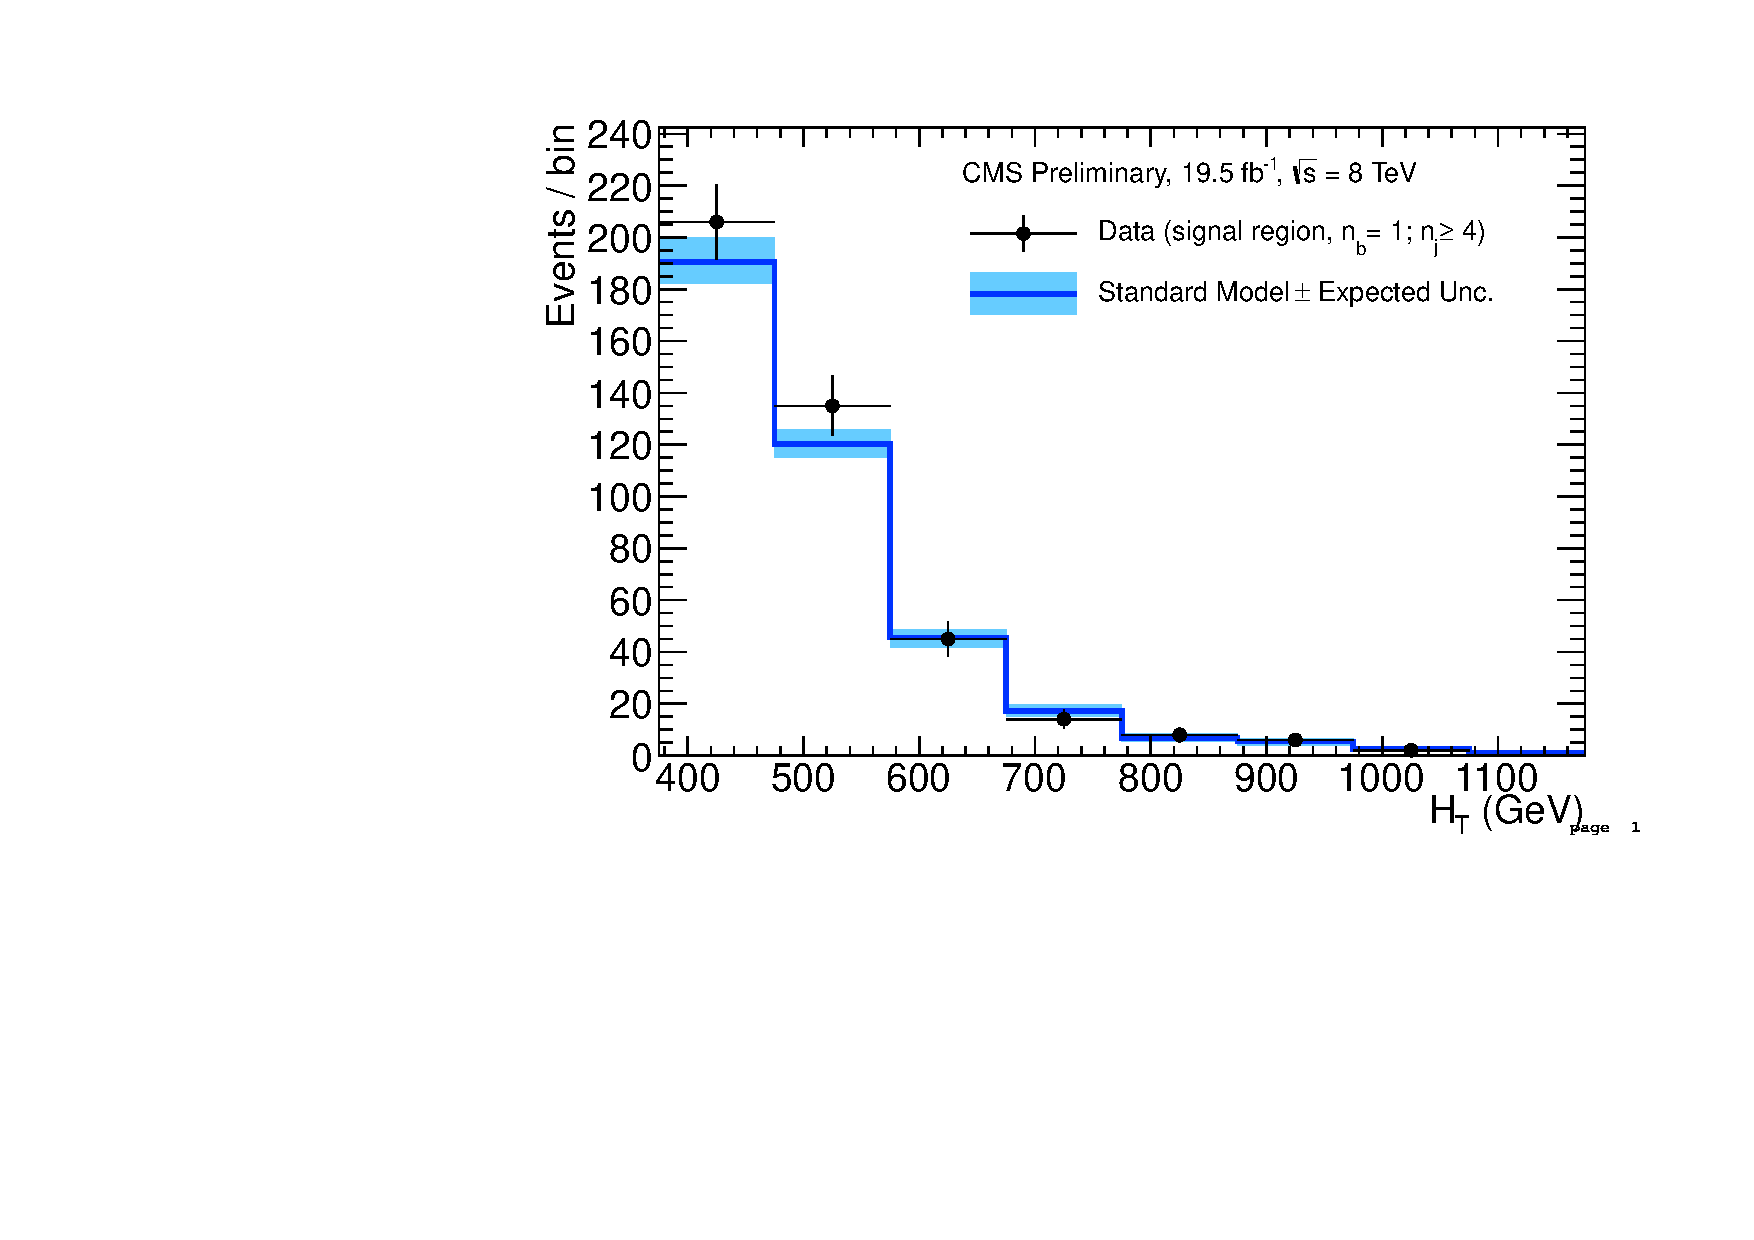
\includegraphics[width=0.45\textwidth,page=1]{figures/fit/v22/bestFit_2012pf_RQcdZero_fZinvAll_1b_ge4j-1hp_smOnly}
    } 
    \subfigure[Hadronic sample (logarithmic scale)]{
      \includegraphics[width=0.45\textwidth,page=2]{figures/fit/v22/bestFit_2012pf_RQcdZero_fZinvAll_1b_ge4j-1hp_smOnly}
    } \\
    \subfigure[$\mu$ + jets sample]{
      \includegraphics[width=0.45\textwidth,page=4]{figures/fit/v22/bestFit_2012pf_RQcdZero_fZinvAll_1b_ge4j-1hp_smOnly}
    } 
    \subfigure[$\gamma$ + jets sample]{
      \includegraphics[width=0.45\textwidth,page=6]{figures/fit/v22/bestFit_2012pf_RQcdZero_fZinvAll_1b_ge4j-1hp_smOnly}
    } 
    \caption{\label{fig:best-fit-ge4j1b} Comparison of the
      \scalht-binned observed data yields and SM expectations when
      requiring \njethigh and $\nb = 1$ for the (a-b) hadronic, (c)
      \mj, (d) \mmj and (e) \gj samples, as determined by a
      simultaneous fit to all data samples under the SM-only
      hypothesis. The observed event yields in data (black dots) and
      the expectations and their uncertainties (dark blue solid line
      with light blue bands), as determined by the simultaneous fit,
      are shown. 
      %For illustrative purposes only, the signal
      %expectations (pink dashed line) for the model \texttt{T2cc} with
      %$m_{\sq} = 250\GeV$ and $m_{\text{LSP}} = 170\GeV$ are stacked
      %on top of the SM expectations.
      }
  \end{center}
\end{figure}

\clearpage
\begin{figure}[t!]
  \begin{center}
    \subfigure[Hadronic sample (linear scale)]{
      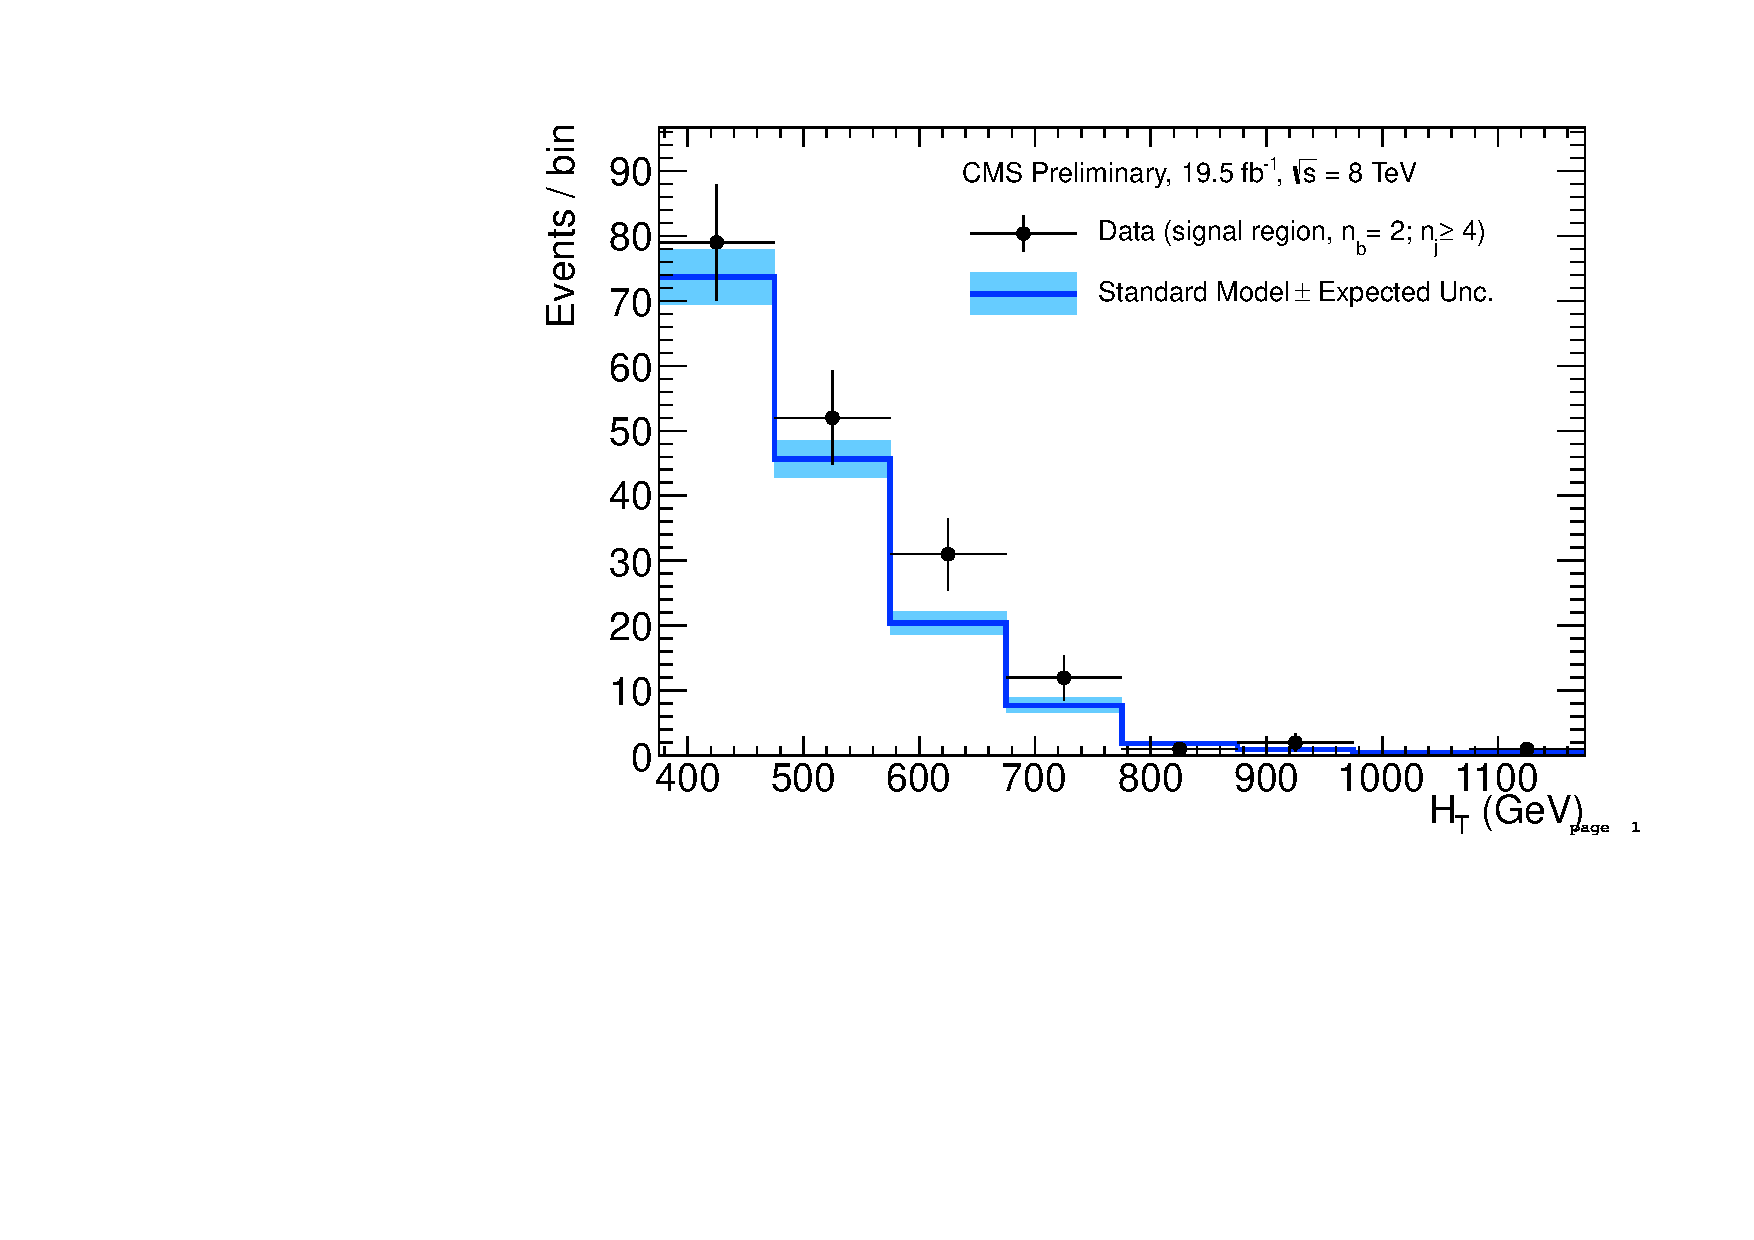
\includegraphics[width=0.45\textwidth,page=1]{figures/fit/v22/bestFit_2012pf_RQcdZero_fZinvAll_2b_ge4j-1h_smOnly}
    } 
    \subfigure[Hadronic sample (logarithmic scale)]{
      \includegraphics[width=0.45\textwidth,page=2]{figures/fit/v22/bestFit_2012pf_RQcdZero_fZinvAll_2b_ge4j-1h_smOnly}
    } \\
    \subfigure[$\mu$ + jets sample]{
      \includegraphics[width=0.45\textwidth,page=4]{figures/fit/v22/bestFit_2012pf_RQcdZero_fZinvAll_2b_ge4j-1h_smOnly}
    } 
    \caption{\label{fig:best-fit-ge4j2b} Comparison of the
      \scalht-binned observed data yields and SM expectations when
      requiring \njethigh and $\nb = 2$ for the (a-b) hadronic and \mj
      samples, as determined by a simultaneous fit to both the
      hadronic and \mj data samples under the SM-only hypothesis. The
      observed event yields in data (black dots) and the expectations
      and their uncertainties (dark blue solid line with light blue
      bands), as determined by the simultaneous fit, are shown. }
%      For illustrative purposes only, the signal expectations (pink
%      dashed line) for the model \texttt{T2cc} with $m_{\sq} =
%      250\GeV$ and $m_{\text{LSP}} = 240\GeV$ are stacked on top of
%      the SM expectations.}
  \end{center}
\end{figure}
%
%
%\clearpage
%\begin{figure}[t!]
%  \begin{center}
%    \subfigure[Hadronic sample (linear scale)]{
%      \includegraphics[width=0.45\textwidth,page=1]{figures/fit/v22/bestFit_2012pf_RQcdZero_fZinvAll_3b_ge4j-1h_smOnly}
%    } 
%    \subfigure[Hadronic sample (logarithmic scale)]{
%      \includegraphics[width=0.45\textwidth,page=2]{figures/fit/v22/bestFit_2012pf_RQcdZero_fZinvAll_3b_ge4j-1h_smOnly}
%    } \\
%    \subfigure[$\mu$ + jets sample]{
%      \includegraphics[width=0.45\textwidth,page=4]{figures/fit/v22/bestFit_2012pf_RQcdZero_fZinvAll_3b_ge4j-1h_smOnly}
%    } 
%    \caption{\label{fig:best-fit-ge4j3b} Comparison of the
%      \scalht-binned observed data yields and SM expectations when
%      requiring \njethigh and $\nb = 3$ for the (a-b) hadronic and \mj
%      samples, as determined by a simultaneous fit to both the
%      hadronic and \mj data samples under the SM-only hypothesis. The
%      observed event yields in data (black dots) and the expectations
%      and their uncertainties (dark blue solid line with light blue
%      bands), as determined by the simultaneous fit, are shown. }
%%      For illustrative purposes only, the signal expectations (pink
%%      dashed line) for the model \texttt{T2cc} with $m_{\sq} =
%%      250\GeV$ and $m_{\text{LSP}} = 240\GeV$ are stacked on top of
%%      the SM expectations.}
%  \end{center}
%\end{figure}
%
%
%\clearpage
%\begin{figure}[t!]
%  \begin{center}
%    \subfigure[Hadronic sample (linear scale)]{
%      \includegraphics[width=0.45\textwidth,page=1]{figures/fit/v22/bestFit_2012pf_RQcdZero_fZinvAll_ge4b_ge4j-1h_smOnly}
%    } 
%    \subfigure[Hadronic sample (logarithmic scale)]{
%      \includegraphics[width=0.45\textwidth,page=2]{figures/fit/v22/bestFit_2012pf_RQcdZero_fZinvAll_ge4b_ge4j-1h_smOnly}
%    } \\
%    \subfigure[$\mu$ + jets sample]{
%      \includegraphics[width=0.45\textwidth,page=4]{figures/fit/v22/bestFit_2012pf_RQcdZero_fZinvAll_ge4b_ge4j-1h_smOnly}
%    } 
%    \caption{\label{fig:best-fit-ge4jge4b} Comparison of the
%      \scalht-binned observed data yields and SM expectations when
%      requiring \njethigh and $\nb \geq 4$ for the (a-b) hadronic and \mj
%      samples, as determined by a simultaneous fit to both the
%      hadronic and \mj data samples under the SM-only hypothesis. The
%      observed event yields in data (black dots) and the expectations
%      and their uncertainties (dark blue solid line with light blue
%      bands), as determined by the simultaneous fit, are shown. }
%%      For illustrative purposes only, the signal expectations (pink
%%      dashed line) for the model \texttt{T2cc} with $m_{\sq} =
%%      250\GeV$ and $m_{\text{LSP}} = 240\GeV$ are stacked on top of
%%      the SM expectations.}
%  \end{center}
%\end{figure}

\clearpage
\section{Limits on SMS production cross sections\label{sec:interpretation}}

Upper limits on the production cross section of the two simplified 
SUSY models described in chapter~\ref{sec:signal} are discussed in this
chapter. 

\subsection{Upper Limits}

As described in section~\ref{sec:cls}, for each mass pair, the 
value of the cross section which gives \cls = 0.05 is defined as the 
upper limit. Figure~\ref{fig:upperLimits} shows the expected and observed
upper limits for the SMS models where a stop particle either
decays to a top quark and a neutralino (\texttt{T2tt}) or a charm quark and 
and a neutralino (\texttt{T2cc}). The production and decay modes of the 
simplified models under consideration are summarized in Table~\ref{tab:sms}. 
Also listed are the \njet and \nb bins that are considered for each
interpretation.


%Appendix~\ref{app:gains} shows the expected limits in the model
%\texttt{T1} when considering an inclusive jet multiplicity bin, $\njet
%\geq 2$, just the exclusive jet multiplicity bin, \njethigh, and the
%combination of the two exclusive jet multiplicity bins, \njetlow and
%\njethigh, in the Figs.~\ref{fig:gains-incl}, \ref{fig:gains-high},
%and \ref{fig:gains-both}. Significant gains of are made when
%considering the higher or both exclusive \njet bins, especially in the
%reach to higher LSP masses.

%Experimental uncertainties on the SM background predictions, the
%integrated luminosity measurement, and the total acceptance times
%efficiency of the selection for the considered signal model are
%included in the calculation of the limit.

%Experimental uncertainties on the SM background predictions
%($10-30\%$), the luminosity measurement (4.4\%), and the total
%acceptance times efficiency of the selection for the considered signal
%model (12\%$-$18\%) are included in the calculation of the limit.
%Signal efficiency in the kinematic region defined by $0 <
%m_{\sGlu(\sQua)} - m_{\textrm{LSP}} < 175\gev$ or $m_{\sGlu(\sQua)} <
%300\gev$ is strongly affected by the presence of initial-state
%radiation. We do not consider this region in which direct (\ie,
%non-ISR induced) production is kinematically forbidden due to the
%$\scalht > 275\GeV$ requirement. Given the large associated
%uncertainties, no interpretation is provided for this kinematic
%region. In the case of model \texttt{T1tttt}, for which pair-produced
%gluinos decay to \ttbar pairs and the LSP, the region $0 < m_{\sGlu} -
%m_{\textrm{LSP}} < 400\gev$ is not considered.

\begin{table}[h!]
  \caption{The first two columns specify the model and its
    production and decay. The next column specifies the event
    categories (in terms of \njet and
    \nb) considered for each interpretation. The last 
    two columns indicate the search sensitivity for each model,
    where $m_{\sq(\sGlu)}^{\textrm{best}}$ and
    $m_{\textrm{LSP}}^{\textrm{best}}$ represent the largest mass 
    beyond which no limit can be set for squarks/gluinos and the LSP,
    respectively. The exclusion range for $m_{\sq(\sGlu)}$ is bounded
    from below by the kinematic region considered for each model, as
    defined in the text. The quoted estimates are determined 
    conservatively from the observed exclusion based on the
    theoretical production cross section minus $1\sigma$
    uncertainty. 
    %For model \texttt{T2tt}, the search is at the threshold of
    %sensitivity for the considered ($m_{\sQua},m_{\rm LSP}$) parameter
    %space, as discussed in the text. 
  }  
  \label{tab:sms}
  \centering
  \footnotesize
  \begin{tabular}{ llcccc }
    \hline
    Model
    & Production/decay
    & Event categories
    & Limit plot
%    & $m_{\sq(\sGlu)}^{\textrm{best}}$~(GeV) 
%    & $m_{\textrm{LSP}}^{\textrm{best}}$~(GeV) 
    \\ [0.5ex]
    \hline
    \texttt{T2cc}
    &
    $\textrm{pp}\,\rightarrow\,\sTop\sTop\,\rightarrow\,\textrm{c}\chiz\bar{\textrm{c}}\chiz$
    & ($\le3$,0), ($\ge4$,0), ($\ge4$,1)
    & \ref{fig:upperLimits-t2cc}
%    & 250
%    & 250
    \\
%    \texttt{T1}
%    &
%    $\textrm{pp}\,\rightarrow\,\sGlu\sGlu\,\rightarrow\,\textrm{q}\bar{\textrm{q}}\chiz\textrm{q}\bar{\textrm{q}}\chiz$
%    & $\geq4$
%    & 0
%    & \ref{fig:t1}
%    & 950
%    & 450
%    \\
%    \texttt{T2}
%    & 
%    $\textrm{pp}\,\rightarrow\,\sQua\sQua\,\rightarrow\,\textrm{q}\chiz\bar{\textrm{q}}\chiz$
%    & 2--3
%    & 0
%    & \ref{fig:t2}
%    & 775
%    & 325
%    \\
    \texttt{T2tt} 
    & 
    $\textrm{pp}\,\rightarrow\,\sTop\sTop\,\rightarrow\,\textrm{t}\chiz\bar{\textrm{t}}\chiz$
    & ($\geq4$,1),($\geq4$,2)
    & \ref{fig:upperLimits-t2tt}
%    & 400 
%    & 25
    \\ 
%    \texttt{T2bb}
%    & 
%    $\textrm{pp}\,\rightarrow\,\sBot\sBot\,\rightarrow\,\textrm{b}\chiz\bar{\textrm{b}}\chiz$
%    & 2--3
%    & 1,2
%    & \ref{fig:t2bb}
%    & 600
%    & 200
%    \\
%    \texttt{T1tttt} 
%    &
%    $\textrm{pp}\,\rightarrow\,\sGlu\sGlu\,\rightarrow\,\textrm{t}\bar{\textrm{t}}\chiz\textrm{t}\bar{\textrm{t}}\chiz$ 
%    & $\geq4$
%    & 2,3,$\geq4$
%    & \ref{fig:t1tttt}
%    & 950
%    & 325
%    \\
%    \texttt{T1bbbb} 
%    & 
%    $\textrm{pp}\,\rightarrow\,\sGlu\sGlu\,\rightarrow\,\textrm{b}\bar{\textrm{b}}\chiz\textrm{b}\bar{\textrm{b}}\chiz$
%    & $\geq4$
%    & 2,3,$\geq4$
%    & \ref{fig:t1bbbb}
%    & 1125
%    & 650
%    \\
    \hline
  \end{tabular}
\end{table}

%\fixme{TEXT REFLECTS USUAL PRESENTATION OF LIMIT PLOTS - ALL RELEVANT
%  INFORMATION IN SHOWN IN REFERENCED FIGURES FOR T2CC - TO BE UPDATED.}
%Figures~\ref{fig:limits-t2cc-exp} and \ref{fig:limits-t2cc-obs} show
%the upper limit on the cross section at 95\% CL as a function of
%$m_{\sq}$ or $m_{\gl}$ and $m_{\rm LSP}$ for various simplified
%models. The point-to-point fluctuations are due to the finite number
%of pseudo-experiments used to determine the observed upper limit. The
%solid thick black line indicates the observed exclusion region
%assuming NLO+NLL~\cite{Beenakker:1996ch, susy-nlo-nll} SUSY cross
%section for squark pair production in the limit of very massive
%gluinos (or vice versa). The thin black lines represent the observed
%excluded region when varying the cross section by its theoretical
%uncertainty. The dashed purple lines indicate the median (thick line)
%$\pm 1 \sigma$ (thin lines) expected exclusion regions.
%
%%Figure~\ref{fig:t2cc-1d} shows the observed upper limit at 95\% CL on
%%the production cross section as a function of the top squark mass
%%($m_{\sTop}$) for the model \texttt{T2cc} when considering two
%%different \sTop-\chiz mass splittings of $\Delta m = 10\gev$ (left)
%%and $\Delta m = 80\gev$ (right). The observed upper limit (95\% CL) on
%%the production cross section is shown as a function of $m_{\sTop}$
%%(solid line), along with the expected upper limit and
%%$\mathbf{\pm2}\sigma$ {\bf experimental uncertainties} (long-dashed
%%line with shaded band), and the NLO+NLL top squark pair-production
%%cross section and theoretical uncertainties (dotted line with shaded
%%band).
%
%Figure~\ref{fig:t2cc-best-fit} shows the \scalht-binned observed data
%yields and expectations for the hadronic sample, as determined by a
%simultaneous fit to all data samples under the signal+background
%hypothesis. The observed event yields in data (black dots), the SM
%expectations (dark blue) and the sum of the SM backgrounds and signal
%expectation (pink) are shown. The signal expectations are for the best
%fit model \texttt{T2cc} with $m_{\sq} = 250\GeV$ and $m_{\text{LSP}} =
%230\GeV$. Three event categories are considered by the fit: (Top)
%\njetlow and $\nb = 0$, (Middle) \njethigh and $\nb = 0$, (Bottom)
%\njethigh and $\nb = 1$. The fit is performed (Left) for each
%individual event category or (Right) simultaneously across all three
%event categories.
%
%\begin{figure}[h!]
%  \begin{center}
%    \subfigure[$+1\sigma$ experimental, relative]{
%      \includegraphics[width=0.45\textwidth,page=3,trim=40 50 20 70,clip=true]{figures/limits/v0/exp/CLs_frequentist_T2cc_2012dev_0b_le3j_0b_ge4j_1b_ge4j_xsLimit_relative}
%    } \quad
%    \subfigure[$+1\sigma$ experimental, excluded points]{
%      \includegraphics[width=0.45\textwidth,page=3,trim=40 50 20 70,clip=true]{figures/limits/v0/exp/CLs_frequentist_T2cc_2012dev_0b_le3j_0b_ge4j_1b_ge4j_xsLimit_simpleExcl}
%    } \\
%    \subfigure[Nominal, relative]{
%      \includegraphics[width=0.45\textwidth,page=1,trim=40 50 20 70,clip=true]{figures/limits/v0/exp/CLs_frequentist_T2cc_2012dev_0b_le3j_0b_ge4j_1b_ge4j_xsLimit_relative}
%    } \quad 
%    \subfigure[Nominal, excluded points]{
%      \includegraphics[width=0.45\textwidth,page=1,trim=40 50 20 70,clip=true]{figures/limits/v0/exp/CLs_frequentist_T2cc_2012dev_0b_le3j_0b_ge4j_1b_ge4j_xsLimit_simpleExcl}
%    } \\
%    \subfigure[$-1\sigma$ experimental, relative]{
%      \includegraphics[width=0.45\textwidth,page=2,trim=40 50 20 70,clip=true]{figures/limits/v0/exp/CLs_frequentist_T2cc_2012dev_0b_le3j_0b_ge4j_1b_ge4j_xsLimit_relative}
%    } \quad 
%    \subfigure[$-1\sigma$ experimental, excluded points]{
%      \includegraphics[width=0.45\textwidth,page=2,trim=40 50 20 70,clip=true]{figures/limits/v0/exp/CLs_frequentist_T2cc_2012dev_0b_le3j_0b_ge4j_1b_ge4j_xsLimit_simpleExcl}
%    } \\
%    \caption{\label{fig:limits-t2cc-exp} \fixme{TEMPORARY PLACE
%        HOLDERS FOR THE FINAL LIMIT PLOT. HOWEVER, ALL RELEVANT
%        INFORMATION IS CONTAINED HERE.} Expected limits for the model 
%      \texttt{T2cc}. In the left column, the plots show the upper
%      limit on the production cross section relative to the
%      theoretical value. In the right column, the plots show the mass
%      points that are excluded (marked red). In all plots, the yellow
%      line should be ignored. The expected limits are shown in the
%      middle row, with limits corresponding to the $+1\sigma$ and
%      $+1\sigma$ variations in the experimental uncertainties shown
%      top and bottom, respectively. }
%  \end{center}
%\end{figure}
%
\begin{figure}[h!]
  \begin{center}
    \subfigure[\njethigh, $\nb = 1$, simultaneous fit,\label{fig:upperLimits-t2cc}]{
      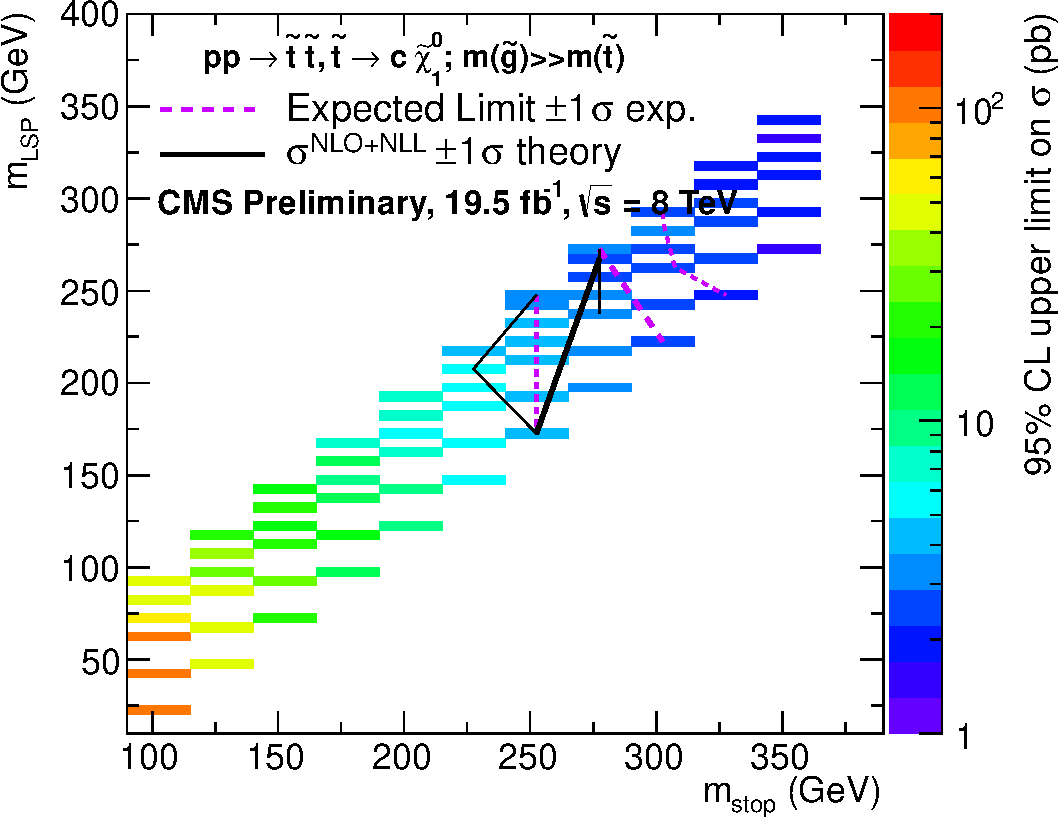
\includegraphics[width=0.70\textwidth,clip=true]{figures/limits/merged/T2cc/v2/CLs_frequentist_T2cc_2012pf_0b_le3j_0b_ge4j_1b_ge4j_xsLimit}
      }\\
    \subfigure[\njethigh, $\nb = 1$, simultaneous fit,\label{fig:upperLimits-t2tt}]{
      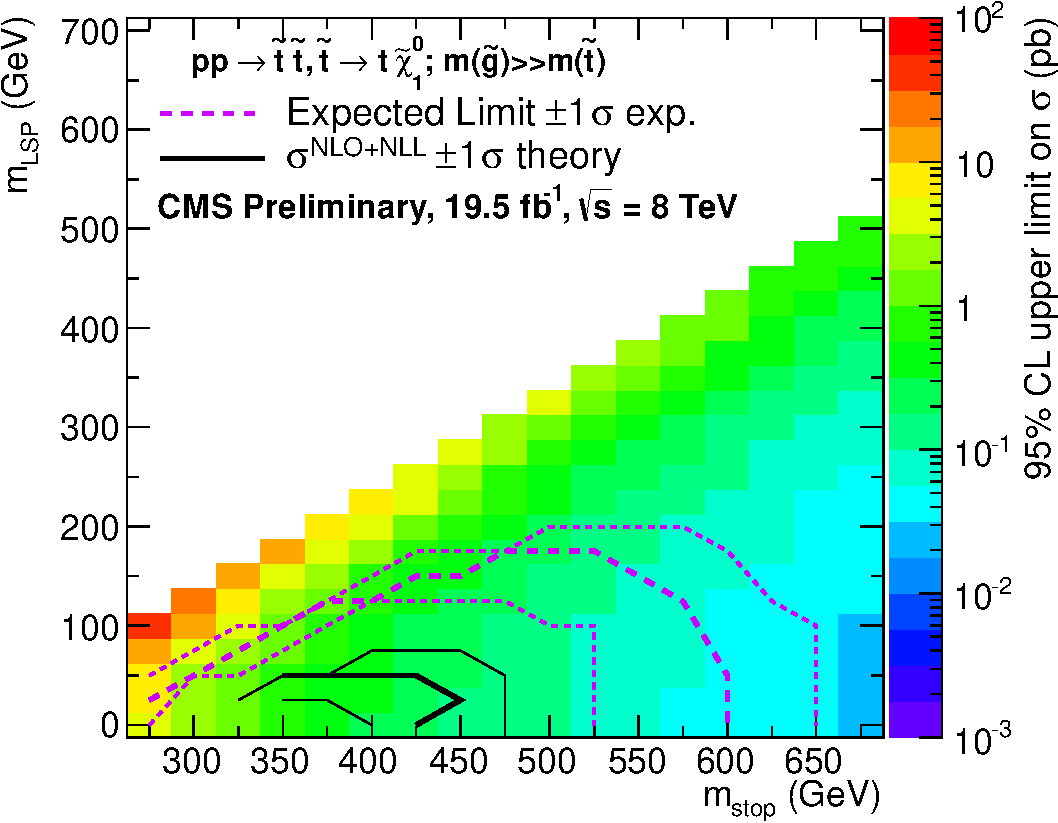
\includegraphics[width=0.70\textwidth,clip=true,]{figures/limits/merged/T2tt/v6/CLs_frequentist_T2tt_2012pf_1b_ge4j_2b_ge4j_xsLimit}
      }
%    \subfigure[Observed, relative]{
%      \includegraphics[width=0.45\textwidth,page=4,trim=40 50 20 70,clip=true]{figures/limits/v0/obs/CLs_frequentist_T2cc_2012dev_0b_le3j_0b_ge4j_1b_ge4j_xsLimit_relative}
%    } \quad 
%    \subfigure[Observed, excluded points]{
%      \includegraphics[width=0.45\textwidth,page=4,trim=40 50 20 70,clip=true]{figures/limits/v0/obs/CLs_frequentist_T2cc_2012dev_0b_le3j_0b_ge4j_1b_ge4j_xsLimit_simpleExcl}
%    } \\
    \caption{\label{fig:upperLimits} Expected 
    and observed upper limits on the production cross section 
    for the for the models \texttt{T2cc} (top) and \texttt{T2tt} (bottom). }
  \end{center}
\end{figure}

\begin{figure*}[t!]
  \begin{center}
    \subfigure[\njethigh, $\nb = 1$, simultaneous fit]{
      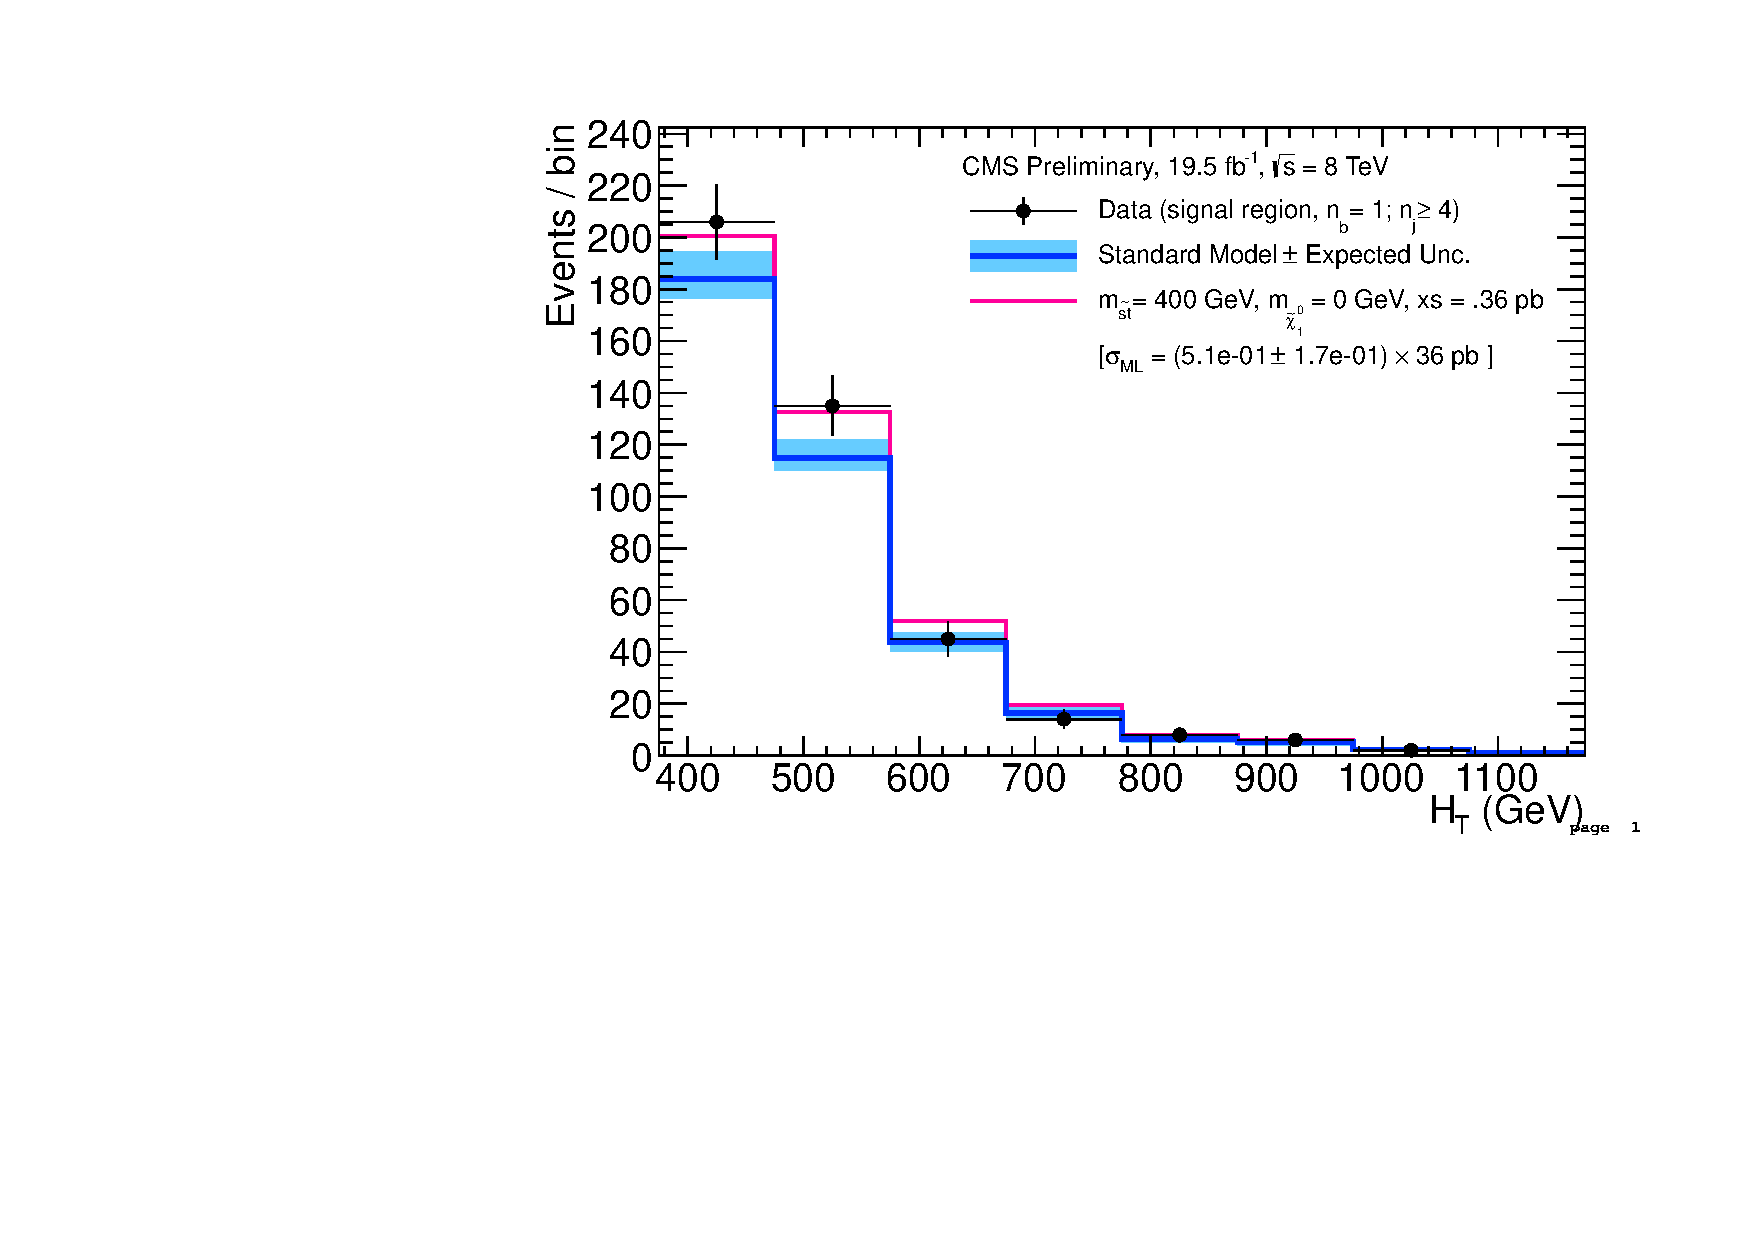
\includegraphics[width=0.45\textwidth]{figures/fit/v22/wSignal/400_0/bestFit_2012pf_RQcdZero_fZinvAll_1b_ge4j-1hp_2b_ge4j-1h_signal_sel1b_ge4j}
    } 
    \subfigure[\njethigh, $\nb = 2$, simultaneous fit]{
      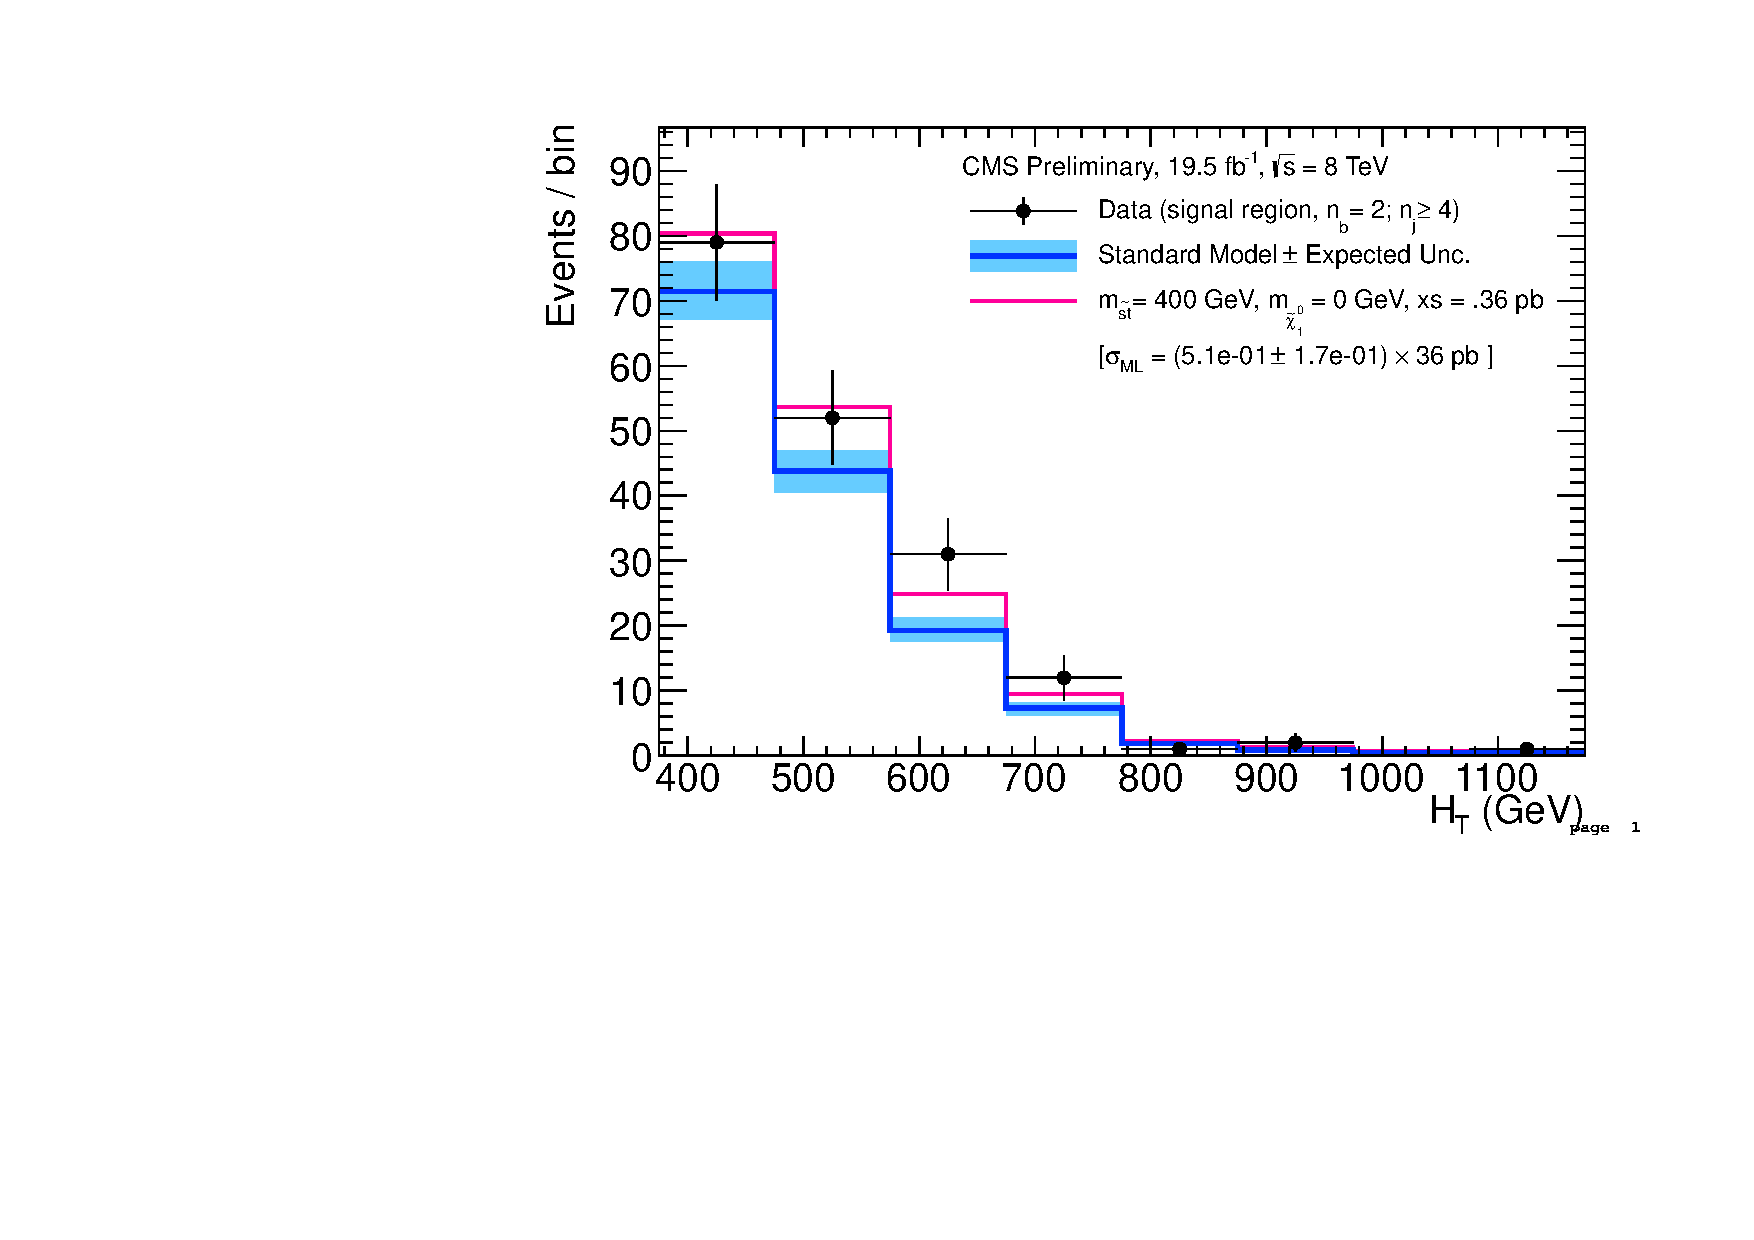
\includegraphics[width=0.45\textwidth]{figures/fit/v22/wSignal/400_0/bestFit_2012pf_RQcdZero_fZinvAll_1b_ge4j-1hp_2b_ge4j-1h_signal_sel2b_ge4j}
    } \\
    \caption{\label{fig:t2cc-best-fit}The comparison of
      the \scalht-binned observed data yields and expectations for the
      hadronic sample, as determined by a simultaneous fit to all data
      samples under the signal plus SM background hypothesis. The
      observed event yields in data (black dots), the SM expectations
      (dark blue solid line), and the signal expectations (pink solid
      line), as determined by the simultaneous fit, for the 
      signal model \texttt{T2tt} with $m_{\st} = 400\GeV$ and
      $m_{\text{LSP}} = 0\GeV$. Two event categories are
      considered: (a) \njethigh and $\nb = 1$, (b) \njethigh and
      $\nb = 2$.}
  \end{center}
\end{figure*}
\begin{figure*}[t!]
  \begin{center}
    \subfigure[profile likelihood ratio, simultaneous fit]{
      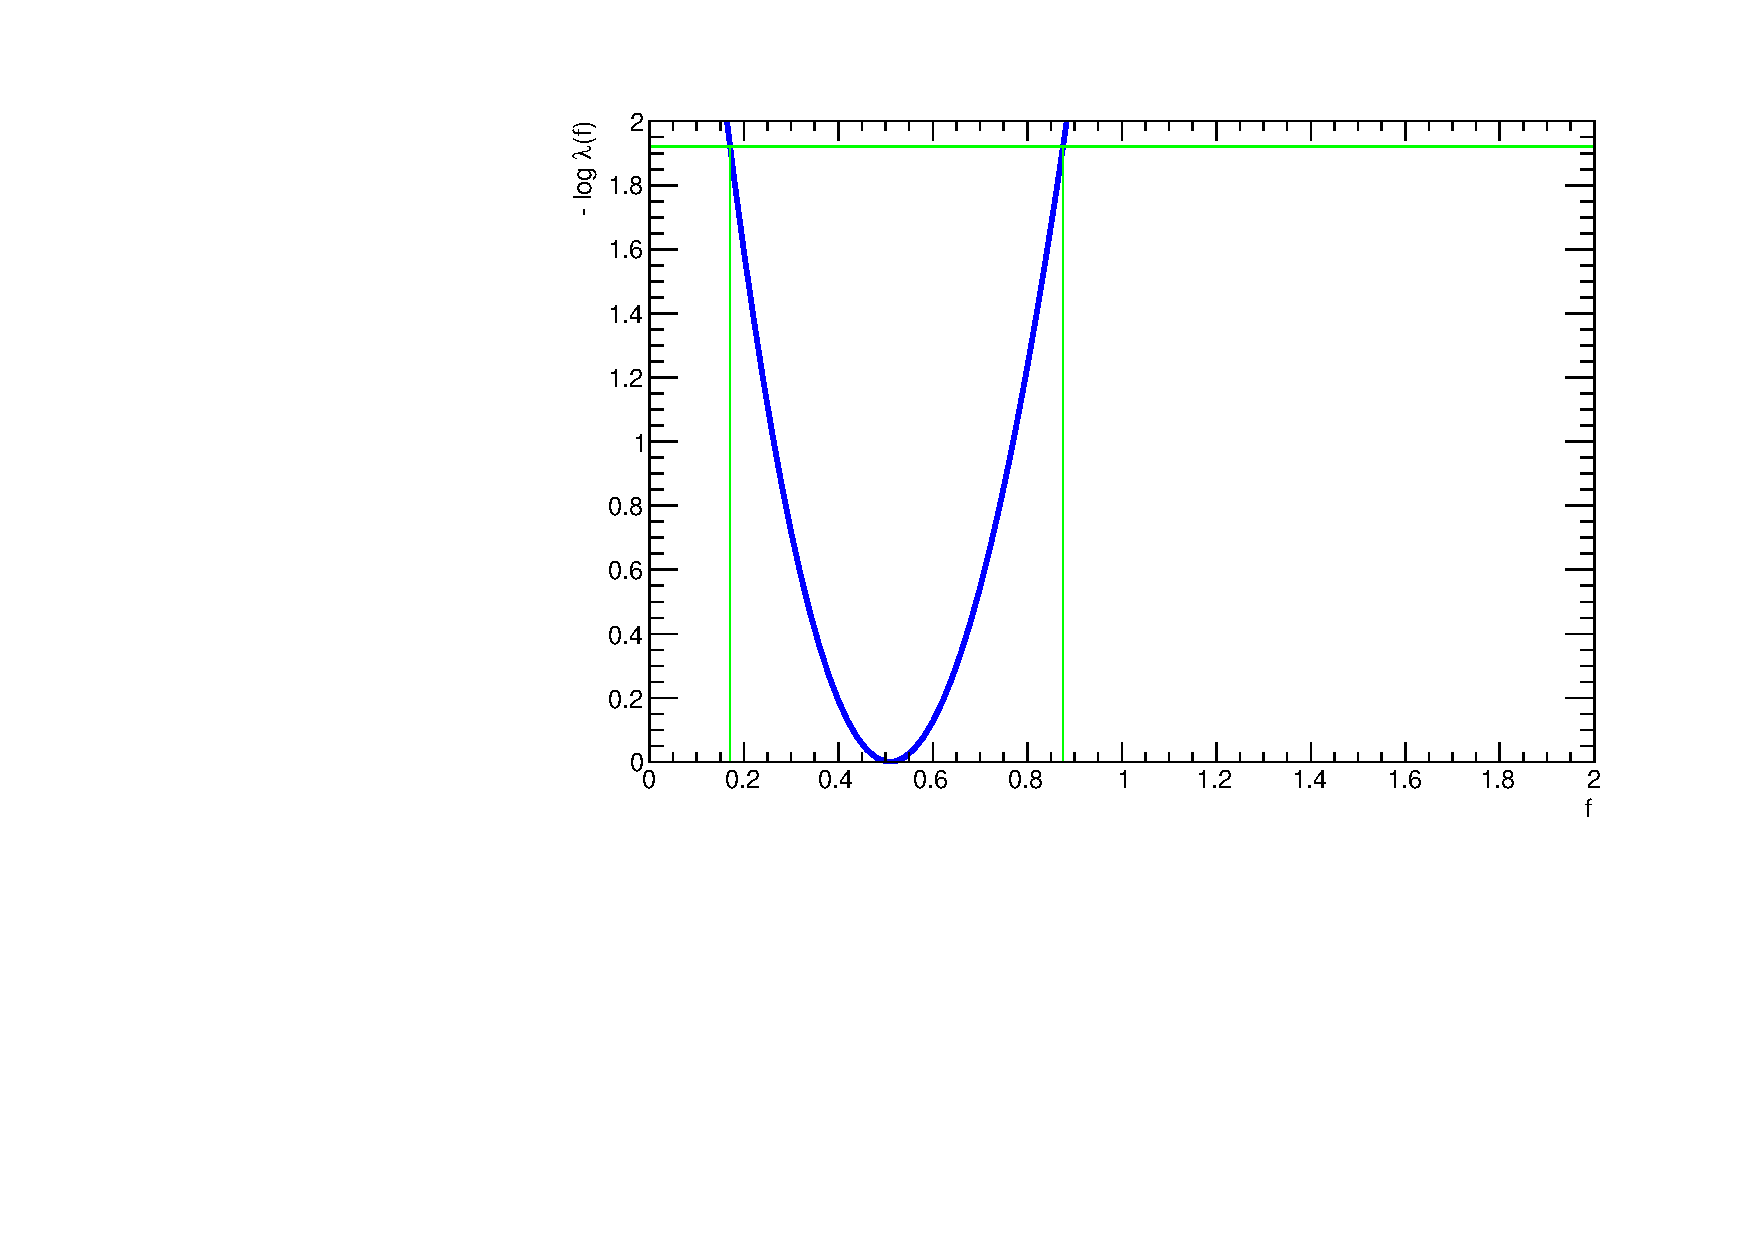
\includegraphics[width=0.45\textwidth]{figures/fit/v22/wSignal/400_0/intervalPlot_2012pf_RQcdZero_fZinvAll_1b_ge4j-1hp_2b_ge4j-1h_signal_95}
    } \\
    \caption{\label{fig:t2cc-best-fit}The profile likelihood ratio 
      (defined in sec.~\ref{sec:cls}) as a function of the signal strength.
      The likelihood considers all data samples under the signal plus SM 
      background hypothesis for the signal model \texttt{T2tt} with 
      $m_{\st} = 400\GeV$ and $m_{\text{LSP}} = 0\GeV$.
      The minimum defines the signal strength estimate which maximizes the
      likelihood and the green vertical line on the right of the minimum 
      indicates the upper-limit at 95\% confidence level.}
  \end{center}
\end{figure*}

\begin{figure*}[t!]
  \begin{center}
     \subfigure[\njethigh, $\nb = 1$, simultaneous fit]{
      \includegraphics[width=0.45\textwidth,page=13]{figures/fit/v22/stackedSig/400_0/bestFit_2012pf_RQcdZero_fZinvAll_1b_ge4j-1p_2b_ge4j-1_sel1b_ge4j_smOnly.pdf}
    } 
    \subfigure[\njethigh, $\nb = 2$, simultaneous fit]{
      \includegraphics[width=0.45\textwidth,page=9]{figures/fit/v22/stackedSig/400_0/bestFit_2012pf_RQcdZero_fZinvAll_1b_ge4j-1p_2b_ge4j-1_sel2b_ge4j_smOnly.pdf}
    } \\
    \caption{\label{fig:t2cc-best-fit} The \scalht-binned 
      signal significance defined as the signal yield 
      divided by the $\sqrt{b+(.1b)^2}$ where $b$ is the
      SM expectation obtained by a fit to all 
      control data samples under the SM-only background 
      hypothesis for the two categories (a) \njethigh, $\nb = 1$ and (b) 
      \njethigh, $\nb = 2$ simultaneously. 
      The signal model is \texttt{T2tt} with 
      $m_{\st} = 400\GeV$ and $m_{\text{LSP}} = 0\GeV$.} 
  \end{center}
\end{figure*}

\begin{figure*}[t!]
  \begin{center}
    \subfigure[\njethigh, $\nb = 1$, simultaneous fit]{
      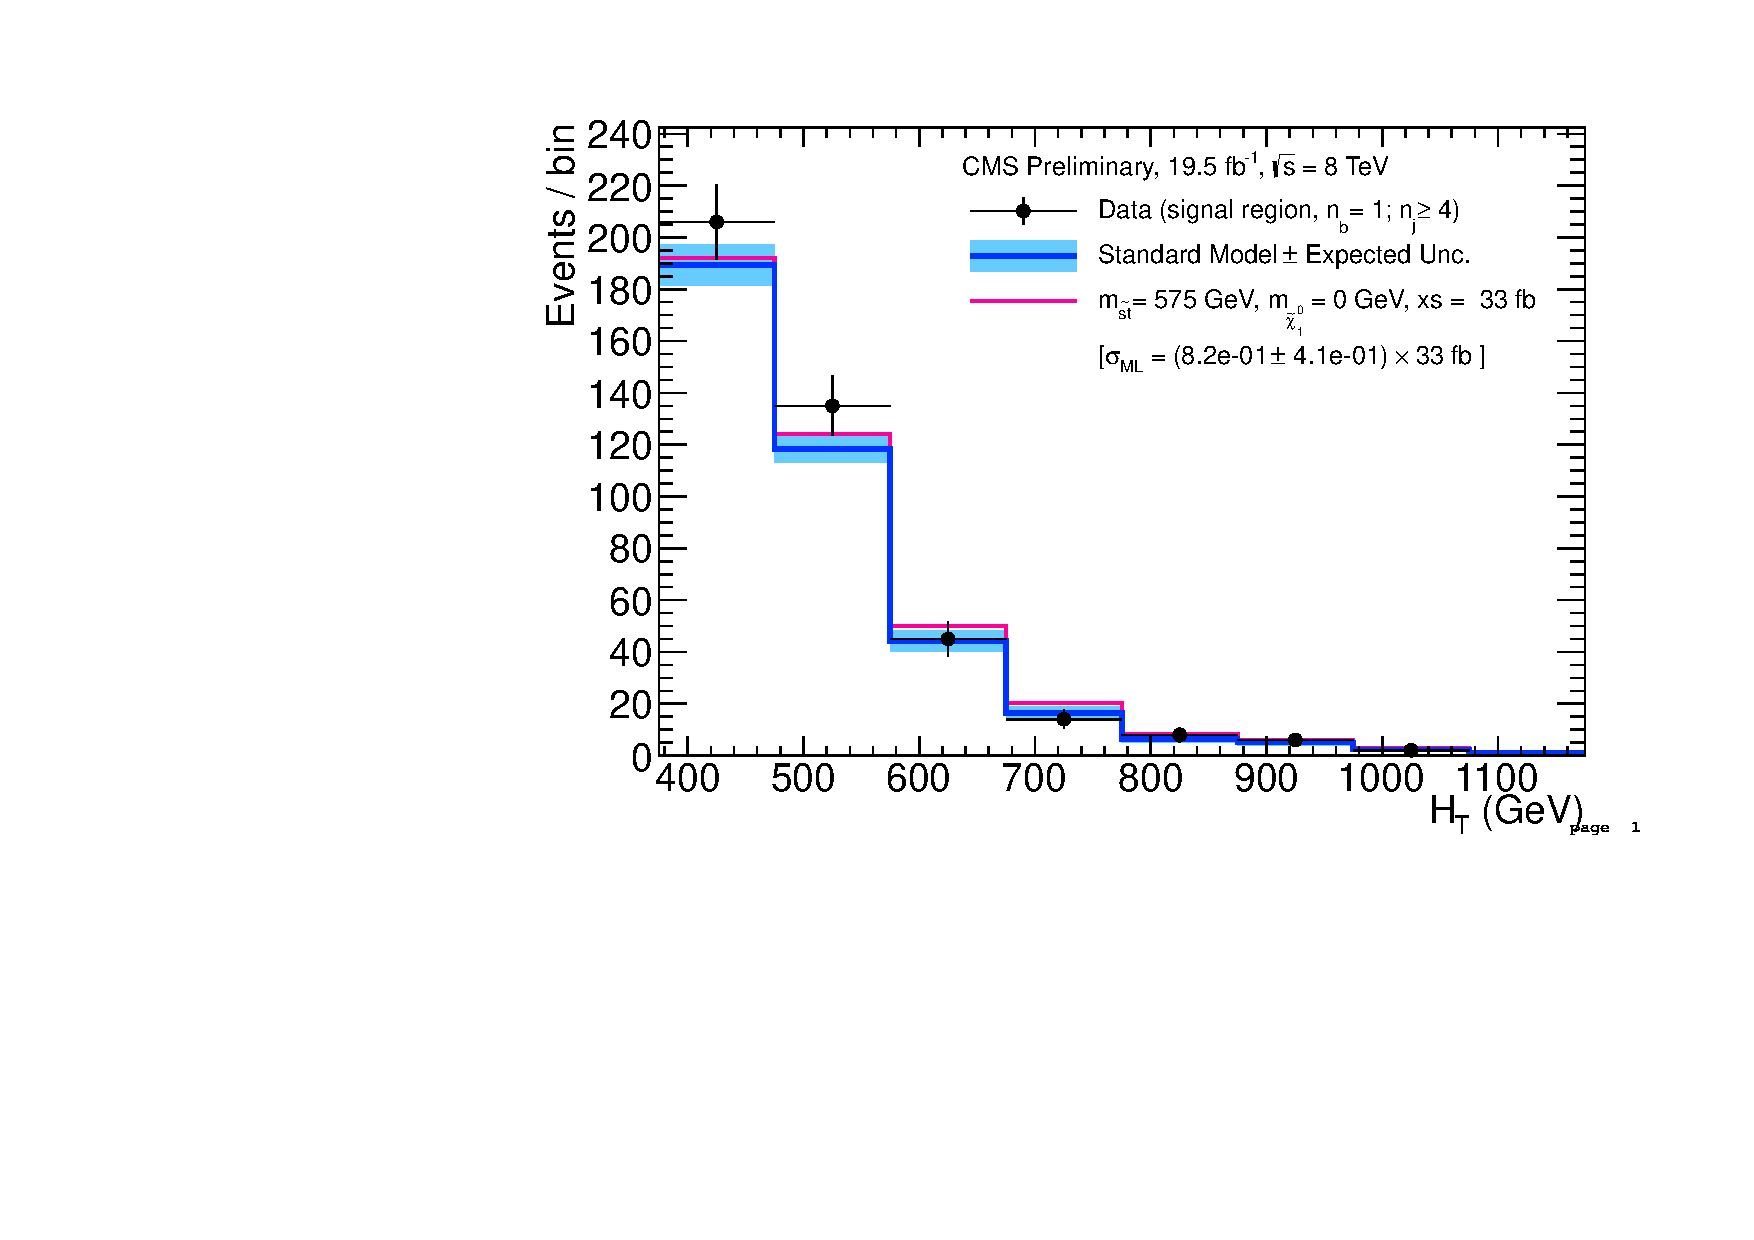
\includegraphics[width=0.45\textwidth]{figures/fit/v22/wSignal/575_0/bestFit_2012pf_RQcdZero_fZinvAll_1b_ge4j-1hp_2b_ge4j-1h_signal_sel1b_ge4j}
    } 
    \subfigure[\njethigh, $\nb = 2$, simultaneous fit]{
      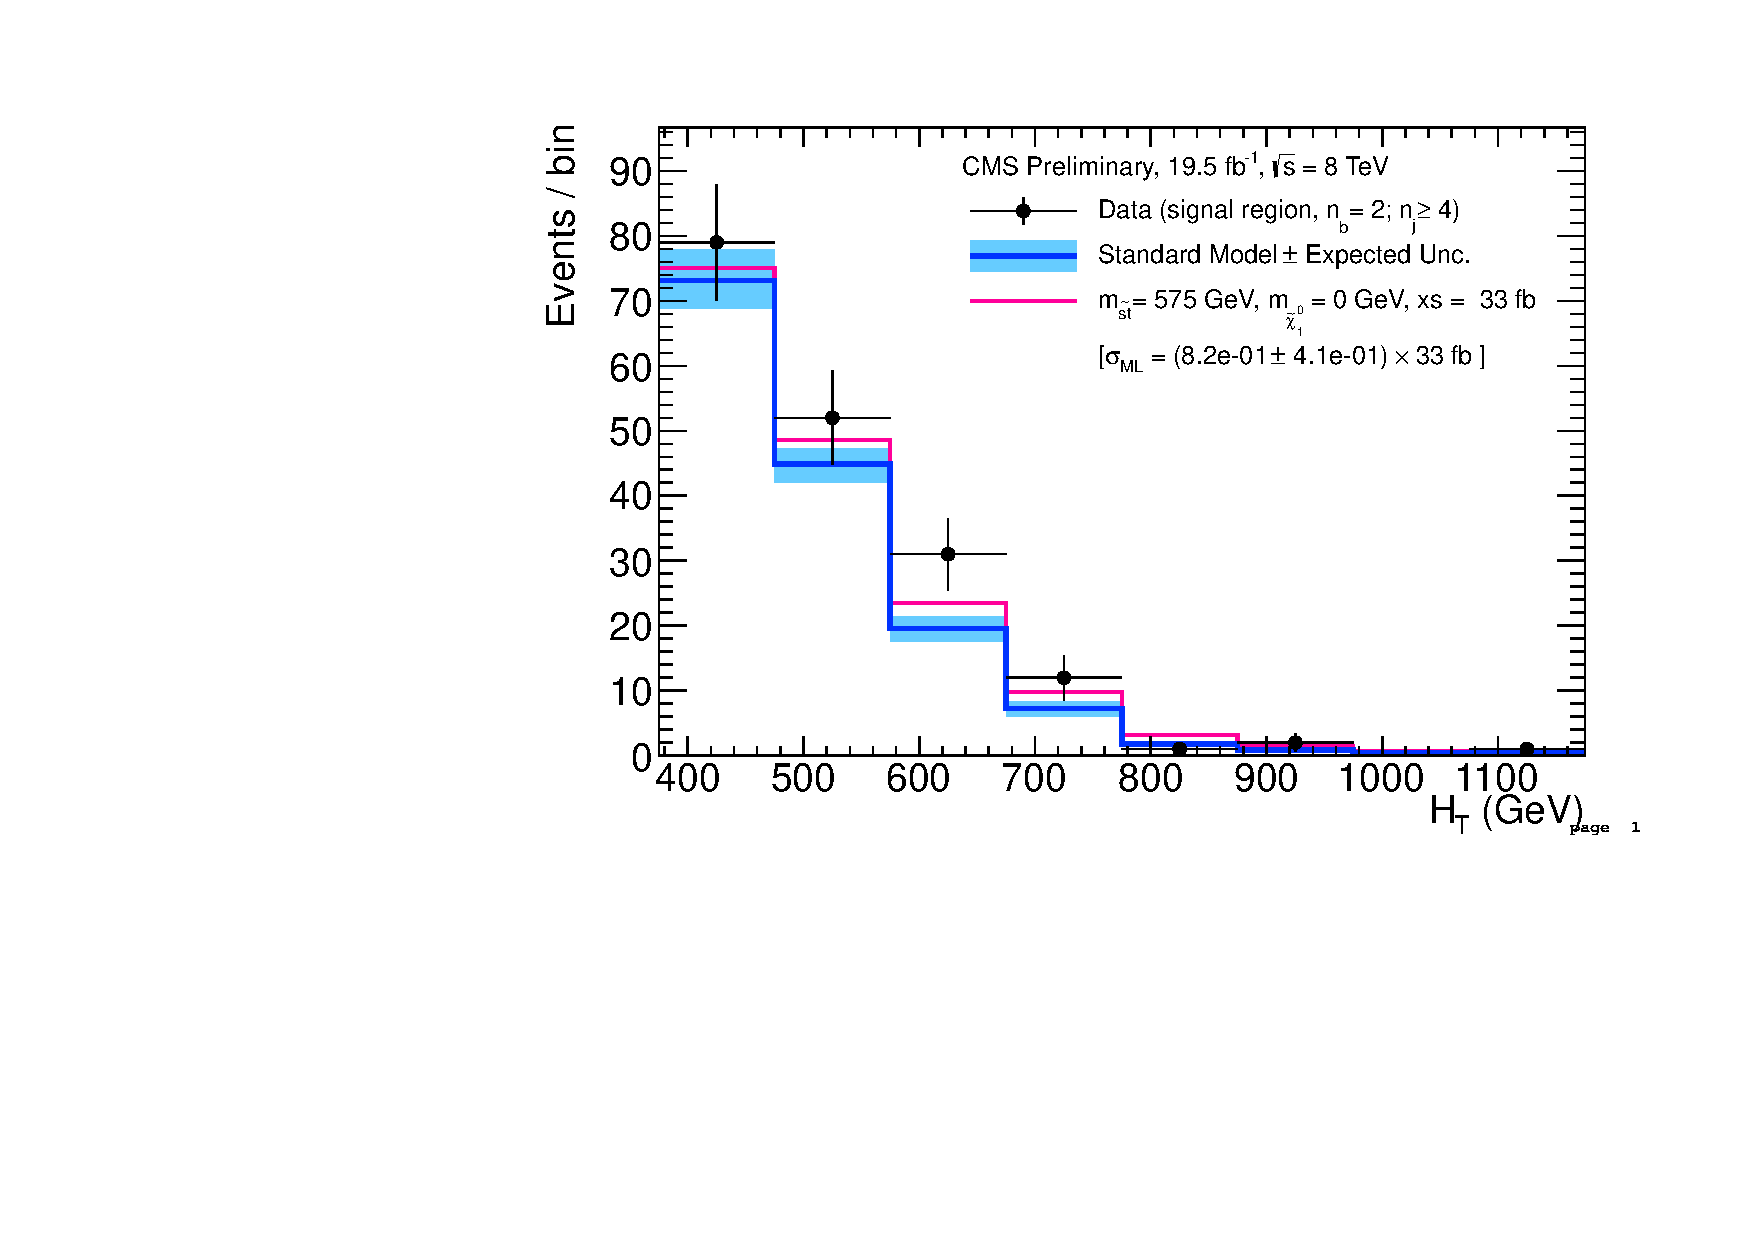
\includegraphics[width=0.45\textwidth]{figures/fit/v22/wSignal/575_0/bestFit_2012pf_RQcdZero_fZinvAll_1b_ge4j-1hp_2b_ge4j-1h_signal_sel2b_ge4j}
    } \\
    \caption{\label{fig:t2cc-best-fit}The comparison of
      the \scalht-binned observed data yields and expectations for the
      hadronic sample, as determined by a simultaneous fit to all data
      samples under the signal plus SM background hypothesis. The
      observed event yields in data (black dots), the SM expectations
      (dark blue solid line), and the signal expectations (pink solid
      line), as determined by the simultaneous fit, for the
      signal model \texttt{T2tt} with $m_{\st} = 575\GeV$ and
      $m_{\text{LSP}} = 0\GeV$. Two event categories are
      considered: (a) \njethigh and $\nb = 1$, (b) \njethigh and
      $\nb = 2$.}
  \end{center}
\end{figure*}
\begin{figure*}[t!]
  \begin{center}
    \subfigure[profile likelihood ratio, simultaneous fit]{
      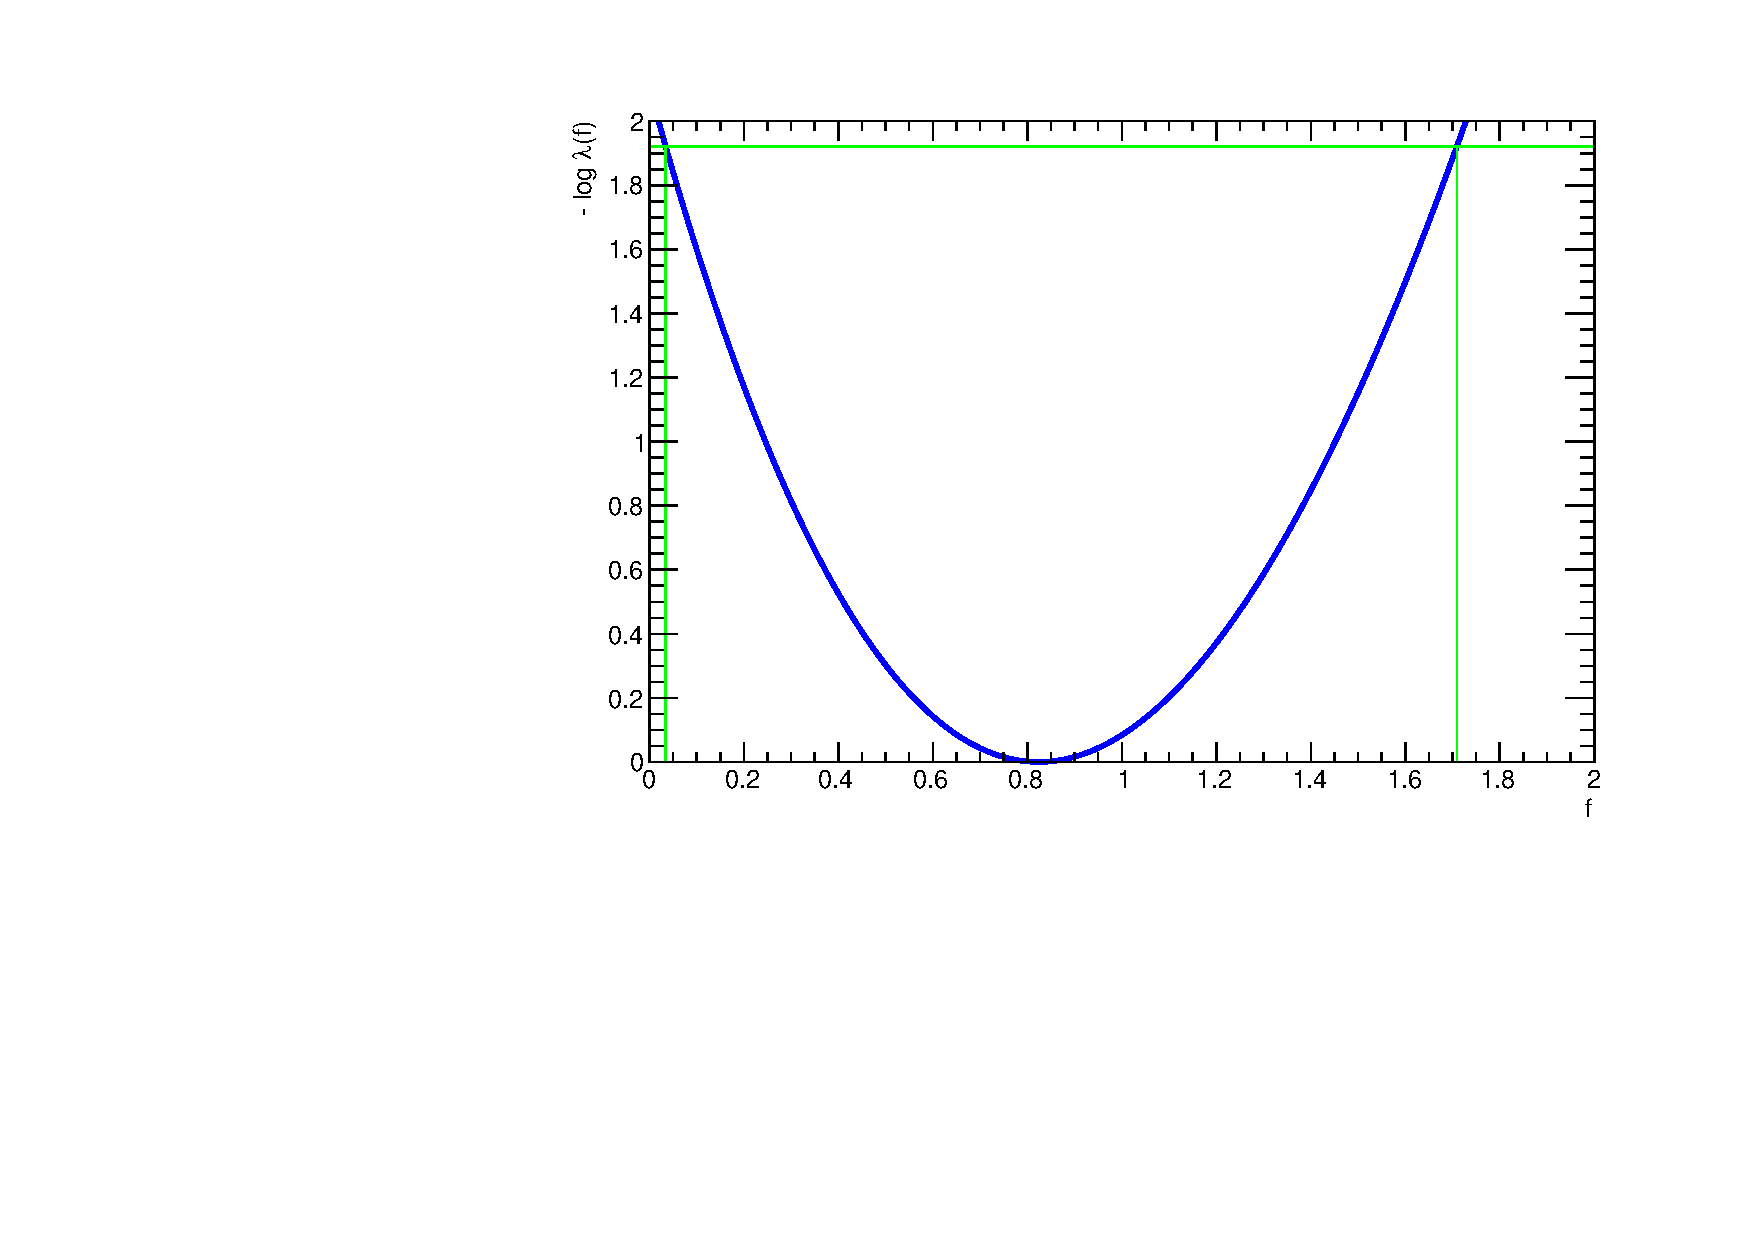
\includegraphics[width=0.45\textwidth]{figures/fit/v22/wSignal/575_0/intervalPlot_2012pf_RQcdZero_fZinvAll_1b_ge4j-1hp_2b_ge4j-1h_signal_95}
    } \\
    \caption{\label{fig:t2cc-best-fit}The profile likelihood ratio 
      (defined in sec.~\ref{sec:cls}) as a function of the signal strength.
      The likelihood considers all data samples under the signal plus SM 
      background hypothesis for the signal model \texttt{T2tt} with 
      $m_{\st} = 575\GeV$ and $m_{\text{LSP}} = 0\GeV$.
      The minimum defines the signal strength estimate which maximizes the
      likelihood and the green vertical line on the right of the minimum 
      indicates the upper-limit at 95\% confidence level.}
  \end{center}
\end{figure*}

\begin{figure*}[t!]
  \begin{center}
     \subfigure[\njethigh, $\nb = 1$, simultaneous fit]{
      \includegraphics[width=0.45\textwidth,page=13]{figures/fit/v22/stackedSig/575_0/bestFit_2012pf_RQcdZero_fZinvAll_1b_ge4j-1p_2b_ge4j-1_sel1b_ge4j_smOnly.pdf}
    } 
    \subfigure[\njethigh, $\nb = 2$, simultaneous fit]{
      \includegraphics[width=0.45\textwidth,page=9]{figures/fit/v22/stackedSig/575_0/bestFit_2012pf_RQcdZero_fZinvAll_1b_ge4j-1p_2b_ge4j-1_sel2b_ge4j_smOnly.pdf}
    } \\
    \caption{\label{fig:t2cc-best-fit} The \scalht-binned 
      signal significance defined as the signal yield 
      divided by the $\sqrt{b+(.1b)^2}$ where $b$ is the
      SM expectation obtained by a fit to all 
      control data samples under the SM-only background 
      hypothesis for the two categories (a) \njethigh, $\nb = 1$ and (b) 
      \njethigh, $\nb = 2$ simultaneously. 
      The signal model is \texttt{T2tt} with 
      $m_{\st} = 575\GeV$ and $m_{\text{LSP}} = 0\GeV$.} 
  \end{center}
\end{figure*}

%%Figure~\ref{fig:limits-sms} shows the upper limit on the cross section
%%at 95\% CL as a function of $m_{\sq}$ or $m_{\gl}$ and $m_{\rm LSP}$
%%for various simplified models. The point-to-point fluctuations are due
%%to the finite number of pseudo-experiments used to determine the
%%observed upper limit. The solid thick black line indicates the
%%observed exclusion region assuming NLO+NLL~\cite{Beenakker:1996ch,
%%  susy-nlo-nll} SUSY cross section for squark pair production in the
%%limit of very massive gluinos (or vice versa). The thin black lines
%%represent the observed excluded region when varying the cross section
%%by its theoretical uncertainty. The dashed purple lines indicate the
%%median (thick line) $\pm 1 \sigma$ (thin lines) expected exclusion
%%regions.
%
%%The estimates on mass limits are determined conservatively from the
%%observed exclusion based on the theoretical production cross section
%%minus $1\sigma$ uncertainty.  The most stringent mass limits on
%%pair-produced sparticles are obtained at low LSP masses, while the
%%limits typically weaken for compressed spectra, \ie, points close to
%%the diagonal. In particular, for all of the considered simplified
%%models, there is an LSP mass beyond which no limit can be set. This is
%%illustrated in Figure~\ref{fig:t1}, where the most stringent limit on
%%the gluino mass of $950\GeV$ is obtained for low LSP masses. This
%%limit only weakens to $900\GeV$ when the LSP mass reaches
%%$425\GeV$. However, for LSP masses above $450\GeV$, no mass range can
%%be excluded for gluinos decaying to first- or second-generation
%%quarks. Table~\ref{tab:sms} summarises the mass limits obtained from
%%the considered simplified models.
%%
%%\begin{figure}[h!]
%%  \begin{center}
%%    \subfigure[\label{fig:t1}$\sGlu\sGlu\,\rightarrow\,\textrm{q}\bar{\textrm{q}}\chiz \textrm{q}\bar{\textrm{q}}\chiz$ (Model \texttt{T1})]{
%%      \includegraphics[width=0.45\textwidth]{figures/limits/v4/t1}
%%    } \quad
%%    \subfigure[\label{fig:t2}$\sQua\sQua\,\rightarrow\,\textrm{q}\chiz \bar{\textrm{q}}\chiz$ (Model \texttt{T2})]{ 
%%      \includegraphics[width=0.45\textwidth]{figures/limits/v4/t2}
%%    } \\
%%%    \subfigure[\label{fig:t2tt}$\sTop\sTop\,\rightarrow\,\textrm{t}\chiz \bar{\textrm{t}}\chiz$ (Model \texttt{T2tt})]{ 
%%%      \includegraphics[width=0.45\textwidth]{figures/limits/v1/t2tt}
%%%    } \quad 
%%    \subfigure[\label{fig:t2bb}$\sBot\sBot\,\rightarrow\,\textrm{b}\chiz \bar{\textrm{b}}\chiz$ (Model \texttt{T2bb})]{ 
%%      \includegraphics[width=0.45\textwidth]{figures/limits/v4/t2bb}
%%    } \\
%%    \subfigure[\label{fig:t1tttt}$\sGlu\sGlu\,\rightarrow\,\textrm{t}\bar{\textrm{t}}\chiz \textrm{t}\bar{\textrm{t}}\chiz$ (Model \texttt{T1tttt})]{
%%      \includegraphics[width=0.45\textwidth]{figures/limits/v4/t1tttt}
%%    } \quad 
%%    \subfigure[\label{fig:t1bbbb}$\sGlu\sGlu\,\rightarrow\,\textrm{b}\bar{\textrm{b}}\chiz \textrm{b}\bar{\textrm{b}}\chiz$ (Model \texttt{T1bbbb})]{
%%      \includegraphics[width=0.45\textwidth]{figures/limits/v4/t1bbbb}
%%    } \\
%%    \caption{\label{fig:limits-sms} Upper limit on cross section at
%%      95\% CL as a function of $m_{\sq}$ or $m_{\gl}$ and $m_{\rm
%%        LSP}$ for various simplified models. The solid thick black
%%      line indicates the observed exclusion region assuming NLO+NLL
%%      SUSY production cross section. The thin black lines represent
%%      the observed excluded region when varying the cross section by
%%      its theoretical uncertainty. The dashed purple lines indicate
%%      the median (thick line) $\pm 1 \sigma$ (thin lines) expected
%%      exclusion regions. 
%%      %The mass ranges considered for models \texttt{T2tt} and
%%      %\texttt{T1tttt} differ from the other models.  
%%    }
%%  \end{center}
%%\end{figure}
%%
%%\begin{figure*}[t!]
%%  \begin{center}
%%    \includegraphics[width=0.45\textwidth]{figures/limits/v4/T2tt_mlsp0_xmin300_smooth5_prelim.pdf} \,
%%    \includegraphics[width=0.45\textwidth]{figures/limits/v4/T2tt_mlsp50_xmin300_smooth5_prelim.pdf}  \\
%%    \includegraphics[width=0.45\textwidth]{figures/limits/v4/T2tt_mlsp100_xmin300_smooth5_prelim.pdf} \,
%%    \includegraphics[width=0.45\textwidth]{figures/limits/v4/T2tt_mlsp150_xmin350_smooth5_prelim.pdf} \\
%%    \caption{\label{fig:t2tt-1d} Excluded cross sections versus top
%%      squark mass $m_{\sTop}$ for the model \texttt{T2tt}, in which
%%      pair-produced top squarks each decay to a top quark and the LSP
%%      with a mass $m_{\rm LSP} = 0\gev$ (top left), $m_{\rm LSP} =
%%      50\gev$ (top right), $m_{\rm LSP} = 100\gev$ (bottom left),
%%      $m_{\rm LSP} = 150\gev$ (bottom right). The observed upper limit
%%      (95\% CL) on the production cross section is shown as a function
%%      of $m_{\sTop}$ (solid line), along with the expected upper limit
%%      and $\pm1\sigma$ experimental uncertainties (long-dashed line
%%      with shaded band), and the NLO+NLL top squark pair-production
%%      cross section and theoretical uncertainties (dotted line with
%%      shaded band).}
%%  \end{center}
%%\end{figure*}
%%
%%Figure~\ref{fig:t2tt-1d} shows the observed upper limit at 95\% CL on
%%the production cross section as a function of the top squark mass
%%($m_{\sTop}$) for the model \texttt{T2tt} when considering different
%%LSP masses in the range 0--150\GeV. No exclusion on possible top
%%squark masses is observed when considering the theoretical production
%%cross section minus $1\sigma$ uncertainty. However, the expected
%%exclusion covers the ranges 300--520\GeV, 320--520\GeV, and
%%420-480\GeV for $m_{\text{LSP}} = 0\GeV$, $m_{\text{LSP}} = 50\GeV$,
%%and $m_{\text{LSP}} = 100\GeV$ respectively. No exclusion is expected
%%for the LSP with a mass greater than 100\GeV.
%%%The expected reach for the T2tt model is summarised
%%%in Table~\ref{tab:sms-reach}. 

%\clearpage
\begin{figure}[t!]
  \begin{center}
    \subfigure[Hadronic sample (linear scale)]{
      \includegraphics[width=0.45\textwidth,page=1]{figures/fit/v21/bestFit_2012pf_RQcdZero_fZinvAll_0b_le3j-1p_smOnly}
    } 
    \subfigure[Hadronic sample (logarithmic scale)]{
      \includegraphics[width=0.45\textwidth,page=2]{figures/fit/v21/bestFit_2012pf_RQcdZero_fZinvAll_0b_le3j-1p_smOnly}
    } \\
    \subfigure[$\mu$ + jets sample]{
      \includegraphics[width=0.45\textwidth,page=4]{figures/fit/v21/bestFit_2012pf_RQcdZero_fZinvAll_0b_le3j-1p_smOnly}
    } 
    \subfigure[$\gamma$ + jets sample]{
      \includegraphics[width=0.45\textwidth,page=6]{figures/fit/v21/bestFit_2012pf_RQcdZero_fZinvAll_0b_le3j-1p_smOnly}
    } 
    \caption{\label{fig:best-fit-control-only-le3j0b} Comparison of the
      \scalht-binned observed data yields and SM expectations
      when requiring \njetlow and $\nb = 0$ for the (a-b) hadronic,
      (c) \mj, (d) \mmj and (e) \gj samples, as determined by a
      simultaneous fit to the data control samples only. The observed
      event yields in data (black dots) and the expectations and their
      uncertainties (dark green solid line with light green bands), as
      determined by the simultaneous fit, are shown. }
%      For illustrative purposes only, the signal expectations (pink
%      dashed line) for the model \texttt{T2cc} with $m_{\sq} =
%      250\GeV$ and $m_{\text{LSP}} = 240\GeV$ are stacked on top of
%      the SM expectations.}
  \end{center}
\end{figure}

\clearpage
\begin{figure}[t!]
  \begin{center}
    \subfigure[Hadronic sample (linear scale)]{
      \includegraphics[width=0.45\textwidth,page=1]{figures/fit/v21/bestFit_2012pf_RQcdZero_fZinvAll_1b_le3j-1p_smOnly}
    } 
    \subfigure[Hadronic sample (logarithmic scale)]{
      \includegraphics[width=0.45\textwidth,page=2]{figures/fit/v21/bestFit_2012pf_RQcdZero_fZinvAll_1b_le3j-1p_smOnly}
    } \\
    \subfigure[$\mu$ + jets sample]{
      \includegraphics[width=0.45\textwidth,page=4]{figures/fit/v21/bestFit_2012pf_RQcdZero_fZinvAll_1b_le3j-1p_smOnly}
    } 
    \subfigure[$\gamma$ + jets sample]{
      \includegraphics[width=0.45\textwidth,page=6]{figures/fit/v21/bestFit_2012pf_RQcdZero_fZinvAll_1b_le3j-1p_smOnly}
    } 
    \caption{\label{fig:best-fit-control-only-le3j1b} Comparison of the
      \scalht-binned observed data yields and SM expectations when
      requiring \njetlow and $\nb = 1$ for the (a-b) hadronic, (c)
      \mj, (d) \mmj and (e) \gj samples, as determined by a
      simultaneous fit to the data control samples only. The observed
      event yields in data (black dots) and the expectations and their
      uncertainties (dark green solid line with light green bands), as
      determined by the simultaneous fit, are shown. }
%      For illustrative purposes only, the signal expectations (pink
%      dashed line) for the model \texttt{T2cc} with $m_{\sq} =
%      250\GeV$ and $m_{\text{LSP}} = 170\GeV$ are stacked on top of
%      the SM expectations.}
  \end{center}
\end{figure}

\clearpage
\begin{figure}[t!]
  \begin{center}
    \subfigure[Hadronic sample (linear scale)]{
      \includegraphics[width=0.45\textwidth,page=1]{figures/fit/v21/bestFit_2012pf_RQcdZero_fZinvAll_2b_le3j-1_smOnly}
    } 
    \subfigure[Hadronic sample (logarithmic scale)]{
      \includegraphics[width=0.45\textwidth,page=2]{figures/fit/v21/bestFit_2012pf_RQcdZero_fZinvAll_2b_le3j-1_smOnly}
    } \\
    \subfigure[$\mu$ + jets sample]{
      \includegraphics[width=0.45\textwidth,page=4]{figures/fit/v21/bestFit_2012pf_RQcdZero_fZinvAll_2b_le3j-1_smOnly}
    } 
    \caption{\label{fig:best-fit-control-only-le3j2b} Comparison of the
      \scalht-binned observed data yields and SM expectations when
      requiring \njetlow and $\nb = 2$ for the (a-b) hadronic, (c)
      \mj, (d) \mmj and (e) \gj samples, as determined by the \mj data
      control sample only. The observed event yields in data (black
      dots) and the expectations and their uncertainties (dark green
      solid line with light green bands) are shown. }
%      For illustrative purposes only, the signal expectations (pink
%      dashed line) for the model \texttt{T2cc} with $m_{\sq} =
%      250\GeV$ and $m_{\text{LSP}} = 240\GeV$ are stacked on top of
%      the SM expectations.}
  \end{center}
\end{figure}

\clearpage
\begin{figure}[t!]
  \begin{center}
    \subfigure[Hadronic sample (linear scale)]{
      \includegraphics[width=0.45\textwidth,page=1]{figures/fit/v21/bestFit_2012pf_RQcdZero_fZinvAll_0b_ge4j-1p_smOnly}
    } 
    \subfigure[Hadronic sample (logarithmic scale)]{
      \includegraphics[width=0.45\textwidth,page=2]{figures/fit/v21/bestFit_2012pf_RQcdZero_fZinvAll_0b_ge4j-1p_smOnly}
    } \\
    \subfigure[$\mu$ + jets sample]{
      \includegraphics[width=0.45\textwidth,page=4]{figures/fit/v21/bestFit_2012pf_RQcdZero_fZinvAll_0b_ge4j-1p_smOnly}
    } 
    \subfigure[$\gamma$ + jets sample]{
      \includegraphics[width=0.45\textwidth,page=6]{figures/fit/v21/bestFit_2012pf_RQcdZero_fZinvAll_0b_ge4j-1p_smOnly}
    } 
    \caption{\label{fig:best-fit-control-only-ge4j0b} Comparison of the
      \scalht-binned observed data yields and SM expectations when
      requiring \njethigh and $\nb = 0$ for the (a-b) hadronic, (c)
      \mj, (d) \mmj and (e) \gj samples, as determined by a
      simultaneous fit to the data control samples only. The observed
      event yields in data (black dots) and the expectations and their
      uncertainties (dark green solid line with light green bands), as
      determined by the simultaneous fit, are shown. }
%      For illustrative purposes only, the signal expectations (pink
%      dashed line) for the model \texttt{T2cc} with $m_{\sq} =
%      250\GeV$ and $m_{\text{LSP}} = 170\GeV$ are stacked on top of
%      the SM expectations.}
  \end{center}
\end{figure}

\clearpage
\begin{figure}[t!]
  \begin{center}
    \subfigure[Hadronic sample (linear scale)]{
      \includegraphics[width=0.45\textwidth,page=1]{figures/fit/v21/bestFit_2012pf_RQcdZero_fZinvAll_1b_ge4j-1p_smOnly}
    } 
    \subfigure[Hadronic sample (logarithmic scale)]{
      \includegraphics[width=0.45\textwidth,page=2]{figures/fit/v21/bestFit_2012pf_RQcdZero_fZinvAll_1b_ge4j-1p_smOnly}
    } \\
    \subfigure[$\mu$ + jets sample]{
      \includegraphics[width=0.45\textwidth,page=4]{figures/fit/v21/bestFit_2012pf_RQcdZero_fZinvAll_1b_ge4j-1p_smOnly}
    } 
    \subfigure[$\gamma$ + jets sample]{
      \includegraphics[width=0.45\textwidth,page=6]{figures/fit/v21/bestFit_2012pf_RQcdZero_fZinvAll_1b_ge4j-1p_smOnly}
    } 
    \caption{\label{fig:best-fit-control-only-ge4j1b} Comparison of the
      \scalht-binned observed data yields and SM expectations when
      requiring \njethigh and $\nb = 1$ for the (a-b) hadronic, (c)
      \mj, (d) \mmj and (e) \gj samples, as determined by a
      simultaneous fit to the data control samples only. The observed
      event yields in data (black dots) and the expectations and their
      uncertainties (dark green solid line with light green bands), as
      determined by the simultaneous fit, are shown. }
%      For illustrative purposes only, the signal expectations (pink
%      dashed line) for the model \texttt{T2cc} with $m_{\sq} =
%      250\GeV$ and $m_{\text{LSP}} = 170\GeV$ are stacked on top of
%      the SM expectations.}
  \end{center}
\end{figure}

\clearpage
\begin{figure}[t!]
  \begin{center}
    \subfigure[Hadronic sample (linear scale)]{
      \includegraphics[width=0.45\textwidth,page=1]{figures/fit/v21/bestFit_2012pf_RQcdZero_fZinvAll_2b_ge4j-1_smOnly}
    } 
    \subfigure[Hadronic sample (logarithmic scale)]{
      \includegraphics[width=0.45\textwidth,page=2]{figures/fit/v21/bestFit_2012pf_RQcdZero_fZinvAll_2b_ge4j-1_smOnly}
    } \\
    \subfigure[$\mu$ + jets sample]{
      \includegraphics[width=0.45\textwidth,page=4]{figures/fit/v21/bestFit_2012pf_RQcdZero_fZinvAll_2b_ge4j-1_smOnly}
    } 
    \caption{\label{fig:best-fit-control-only-ge4j2b} Comparison of the
      \scalht-binned observed data yields and SM expectations when
      requiring \njethigh and $\nb = 2$ for the (a-b) hadronic, (c)
      \mj, (d) \mmj and (e) \gj samples, as determined by the \mj data
      control sample only. The observed event yields in data (black
      dots) and the expectations and their uncertainties (dark green
      solid line with light green bands) are shown. }
%      For illustrative purposes only, the signal expectations (pink
%      dashed line) for the model \texttt{T2cc} with $m_{\sq} =
%      250\GeV$ and $m_{\text{LSP}} = 240\GeV$ are stacked on top of
%      the SM expectations.}
  \end{center}
\end{figure}


%\clearpage
%\begin{figure}[t!]
%  \begin{center}
%    \subfigure[Hadronic sample (linear scale)]{
%      \includegraphics[width=0.45\textwidth,page=1]{figures/fit/v21/bestFit_2012pf_RQcdZero_fZinvAll_3b_ge4j-1_smOnly}
%    } 
%    \subfigure[Hadronic sample (logarithmic scale)]{
%      \includegraphics[width=0.45\textwidth,page=2]{figures/fit/v21/bestFit_2012pf_RQcdZero_fZinvAll_3b_ge4j-1_smOnly}
%    } \\
%    \subfigure[$\mu$ + jets sample]{
%      \includegraphics[width=0.45\textwidth,page=4]{figures/fit/v21/bestFit_2012pf_RQcdZero_fZinvAll_3b_ge4j-1_smOnly}
%    } 
%    \caption{\label{fig:best-fit-control-only-ge4j3b} Comparison of the
%      \scalht-binned observed data yields and SM expectations when
%      requiring \njethigh and $\nb = 3$ for the (a-b) hadronic, (c)
%      \mj, (d) \mmj and (e) \gj samples, as determined by the \mj data
%      control sample only. The observed event yields in data (black
%      dots) and the expectations and their uncertainties (dark green
%      solid line with light green bands) are shown. }
%%      For illustrative purposes only, the signal expectations (pink
%%      dashed line) for the model \texttt{T2cc} with $m_{\sq} =
%%      250\GeV$ and $m_{\text{LSP}} = 240\GeV$ are stacked on top of
%%      the SM expectations.}
%  \end{center}
%\end{figure}
%
%
%\clearpage
%\begin{figure}[t!]
%  \begin{center}
%    \subfigure[Hadronic sample (linear scale)]{
%      \includegraphics[width=0.45\textwidth,page=1]{figures/fit/v21/bestFit_2012pf_RQcdZero_fZinvAll_ge4b_ge4j-1_smOnly}
%    } 
%    \subfigure[Hadronic sample (logarithmic scale)]{
%      \includegraphics[width=0.45\textwidth,page=2]{figures/fit/v21/bestFit_2012pf_RQcdZero_fZinvAll_ge4b_ge4j-1_smOnly}
%    } \\
%    \subfigure[$\mu$ + jets sample]{
%      \includegraphics[width=0.45\textwidth,page=4]{figures/fit/v21/bestFit_2012pf_RQcdZero_fZinvAll_ge4b_ge4j-1_smOnly}
%    } 
%    \caption{\label{fig:best-fit-control-only-ge4jge4b} Comparison of the
%      \scalht-binned observed data yields and SM expectations when
%      requiring \njethigh and $\nb \geq 4$ for the (a-b) hadronic, (c)
%      \mj, (d) \mmj and (e) \gj samples, as determined by the \mj data
%      control sample only. The observed event yields in data (black
%      dots) and the expectations and their uncertainties (dark green
%      solid line with light green bands) are shown. }
%%      For illustrative purposes only, the signal expectations (pink
%%      dashed line) for the model \texttt{T2cc} with $m_{\sq} =
%%      250\GeV$ and $m_{\text{LSP}} = 240\GeV$ are stacked on top of
%%      the SM expectations.}
%  \end{center}
%\end{figure}

